% Options for packages loaded elsewhere
\PassOptionsToPackage{unicode}{hyperref}
\PassOptionsToPackage{hyphens}{url}
\documentclass[
]{book}
\usepackage{xcolor}
\usepackage{amsmath,amssymb}
\setcounter{secnumdepth}{5}
\usepackage{iftex}
\ifPDFTeX
  \usepackage[T1]{fontenc}
  \usepackage[utf8]{inputenc}
  \usepackage{textcomp} % provide euro and other symbols
\else % if luatex or xetex
  \usepackage{unicode-math} % this also loads fontspec
  \defaultfontfeatures{Scale=MatchLowercase}
  \defaultfontfeatures[\rmfamily]{Ligatures=TeX,Scale=1}
\fi
\usepackage{lmodern}
\ifPDFTeX\else
  % xetex/luatex font selection
\fi
% Use upquote if available, for straight quotes in verbatim environments
\IfFileExists{upquote.sty}{\usepackage{upquote}}{}
\IfFileExists{microtype.sty}{% use microtype if available
  \usepackage[]{microtype}
  \UseMicrotypeSet[protrusion]{basicmath} % disable protrusion for tt fonts
}{}
\makeatletter
\@ifundefined{KOMAClassName}{% if non-KOMA class
  \IfFileExists{parskip.sty}{%
    \usepackage{parskip}
  }{% else
    \setlength{\parindent}{0pt}
    \setlength{\parskip}{6pt plus 2pt minus 1pt}}
}{% if KOMA class
  \KOMAoptions{parskip=half}}
\makeatother
\usepackage{color}
\usepackage{fancyvrb}
\newcommand{\VerbBar}{|}
\newcommand{\VERB}{\Verb[commandchars=\\\{\}]}
\DefineVerbatimEnvironment{Highlighting}{Verbatim}{commandchars=\\\{\}}
% Add ',fontsize=\small' for more characters per line
\usepackage{framed}
\definecolor{shadecolor}{RGB}{248,248,248}
\newenvironment{Shaded}{\begin{snugshade}}{\end{snugshade}}
\newcommand{\AlertTok}[1]{\textcolor[rgb]{0.94,0.16,0.16}{#1}}
\newcommand{\AnnotationTok}[1]{\textcolor[rgb]{0.56,0.35,0.01}{\textbf{\textit{#1}}}}
\newcommand{\AttributeTok}[1]{\textcolor[rgb]{0.13,0.29,0.53}{#1}}
\newcommand{\BaseNTok}[1]{\textcolor[rgb]{0.00,0.00,0.81}{#1}}
\newcommand{\BuiltInTok}[1]{#1}
\newcommand{\CharTok}[1]{\textcolor[rgb]{0.31,0.60,0.02}{#1}}
\newcommand{\CommentTok}[1]{\textcolor[rgb]{0.56,0.35,0.01}{\textit{#1}}}
\newcommand{\CommentVarTok}[1]{\textcolor[rgb]{0.56,0.35,0.01}{\textbf{\textit{#1}}}}
\newcommand{\ConstantTok}[1]{\textcolor[rgb]{0.56,0.35,0.01}{#1}}
\newcommand{\ControlFlowTok}[1]{\textcolor[rgb]{0.13,0.29,0.53}{\textbf{#1}}}
\newcommand{\DataTypeTok}[1]{\textcolor[rgb]{0.13,0.29,0.53}{#1}}
\newcommand{\DecValTok}[1]{\textcolor[rgb]{0.00,0.00,0.81}{#1}}
\newcommand{\DocumentationTok}[1]{\textcolor[rgb]{0.56,0.35,0.01}{\textbf{\textit{#1}}}}
\newcommand{\ErrorTok}[1]{\textcolor[rgb]{0.64,0.00,0.00}{\textbf{#1}}}
\newcommand{\ExtensionTok}[1]{#1}
\newcommand{\FloatTok}[1]{\textcolor[rgb]{0.00,0.00,0.81}{#1}}
\newcommand{\FunctionTok}[1]{\textcolor[rgb]{0.13,0.29,0.53}{\textbf{#1}}}
\newcommand{\ImportTok}[1]{#1}
\newcommand{\InformationTok}[1]{\textcolor[rgb]{0.56,0.35,0.01}{\textbf{\textit{#1}}}}
\newcommand{\KeywordTok}[1]{\textcolor[rgb]{0.13,0.29,0.53}{\textbf{#1}}}
\newcommand{\NormalTok}[1]{#1}
\newcommand{\OperatorTok}[1]{\textcolor[rgb]{0.81,0.36,0.00}{\textbf{#1}}}
\newcommand{\OtherTok}[1]{\textcolor[rgb]{0.56,0.35,0.01}{#1}}
\newcommand{\PreprocessorTok}[1]{\textcolor[rgb]{0.56,0.35,0.01}{\textit{#1}}}
\newcommand{\RegionMarkerTok}[1]{#1}
\newcommand{\SpecialCharTok}[1]{\textcolor[rgb]{0.81,0.36,0.00}{\textbf{#1}}}
\newcommand{\SpecialStringTok}[1]{\textcolor[rgb]{0.31,0.60,0.02}{#1}}
\newcommand{\StringTok}[1]{\textcolor[rgb]{0.31,0.60,0.02}{#1}}
\newcommand{\VariableTok}[1]{\textcolor[rgb]{0.00,0.00,0.00}{#1}}
\newcommand{\VerbatimStringTok}[1]{\textcolor[rgb]{0.31,0.60,0.02}{#1}}
\newcommand{\WarningTok}[1]{\textcolor[rgb]{0.56,0.35,0.01}{\textbf{\textit{#1}}}}
\usepackage{longtable,booktabs,array}
\usepackage{calc} % for calculating minipage widths
% Correct order of tables after \paragraph or \subparagraph
\usepackage{etoolbox}
\makeatletter
\patchcmd\longtable{\par}{\if@noskipsec\mbox{}\fi\par}{}{}
\makeatother
% Allow footnotes in longtable head/foot
\IfFileExists{footnotehyper.sty}{\usepackage{footnotehyper}}{\usepackage{footnote}}
\makesavenoteenv{longtable}
\usepackage{graphicx}
\makeatletter
\newsavebox\pandoc@box
\newcommand*\pandocbounded[1]{% scales image to fit in text height/width
  \sbox\pandoc@box{#1}%
  \Gscale@div\@tempa{\textheight}{\dimexpr\ht\pandoc@box+\dp\pandoc@box\relax}%
  \Gscale@div\@tempb{\linewidth}{\wd\pandoc@box}%
  \ifdim\@tempb\p@<\@tempa\p@\let\@tempa\@tempb\fi% select the smaller of both
  \ifdim\@tempa\p@<\p@\scalebox{\@tempa}{\usebox\pandoc@box}%
  \else\usebox{\pandoc@box}%
  \fi%
}
% Set default figure placement to htbp
\def\fps@figure{htbp}
\makeatother
\setlength{\emergencystretch}{3em} % prevent overfull lines
\providecommand{\tightlist}{%
  \setlength{\itemsep}{0pt}\setlength{\parskip}{0pt}}
\usepackage[]{natbib}
\bibliographystyle{plainnat}
\usepackage{booktabs}
\usepackage{bookmark}
\IfFileExists{xurl.sty}{\usepackage{xurl}}{} % add URL line breaks if available
\urlstyle{same}
\hypersetup{
  pdftitle={Corner Solution and Count Models},
  pdfauthor={Samuel Rowe adapted from Wooldridge (2011) and Mitchell (2020)},
  hidelinks,
  pdfcreator={LaTeX via pandoc}}

\title{Corner Solution and Count Models}
\author{Samuel Rowe adapted from Wooldridge (2011) and Mitchell (2020)}
\date{2025-09-18}

\begin{document}
\maketitle

{
\setcounter{tocdepth}{1}
\tableofcontents
}
\begin{Shaded}
\begin{Highlighting}[]
\NormalTok{bookdown}\SpecialCharTok{::}\FunctionTok{render\_book}\NormalTok{()}
\end{Highlighting}
\end{Shaded}

\chapter*{Overview}\label{overview}
\addcontentsline{toc}{chapter}{Overview}

This week we will cover corner solutions with a Tobit regresion, and count models with Poisson regression and Negative Binomial regression. For data management, we will cover working within subsets or subsgroups.

\begin{enumerate}
\def\labelenumi{\arabic{enumi}.}
\tightlist
\item
  Corner Solution (Tobit)
\item
  Poisson
\item
  Negative Binominal
\item
  Working with subgroups
\end{enumerate}

\chapter{Corner Solution - Tobit Model}\label{corner-solution---tobit-model}

\section*{Married Women's Annual Labor Supply}\label{married-womens-annual-labor-supply}
\addcontentsline{toc}{section}{Married Women's Annual Labor Supply}

\textbf{Lesson:}
1. Tobit and OLS have the same sign;
2. Tobit and OLS magnitudes are not directly comparable. We need an adjustment factor, or use marginal effects.

We'll look at hours of labor being supplied. We have data on married women' annual labor supply with hours of work for wage in the labor force. There are 428 women employed with hours, and 325
women have no hours. Since we have a sizable about of 0 (corner soluation), we can use a Tobit model.

Summarize hours

\begin{Shaded}
\begin{Highlighting}[]
\NormalTok{cd }\StringTok{"/Users/Sam/Desktop/Econ 645/Data/Wooldridge"}
\KeywordTok{use}\NormalTok{ mroz.dta, }\KeywordTok{clear}
\KeywordTok{sum}\NormalTok{ hours}
\KeywordTok{tab}\NormalTok{ inlf, }\KeywordTok{sum}\NormalTok{(hours)}
\KeywordTok{tab}\NormalTok{ hours }\KeywordTok{if}\NormalTok{ hours == 0}
\KeywordTok{tabstat}\NormalTok{ hours, }\KeywordTok{by}\NormalTok{(inlf) stat(}\KeywordTok{mean} \KeywordTok{median} \FunctionTok{sd}\NormalTok{)}
\end{Highlighting}
\end{Shaded}

\begin{verbatim}
/Users/Sam/Desktop/Econ 645/Data/Wooldridge

    Variable |        Obs        Mean    Std. Dev.       Min        Max
-------------+---------------------------------------------------------
       hours |        753    740.5764    871.3142          0       4950

            |          Summary of hours
       inlf |        Mean   Std. Dev.       Freq.
------------+------------------------------------
          0 |           0           0         325
          1 |   1302.9299   776.27438         428
------------+------------------------------------
      Total |   740.57636   871.31422         753

      hours |      Freq.     Percent        Cum.
------------+-----------------------------------
          0 |        325      100.00      100.00
------------+-----------------------------------
      Total |        325      100.00


Summary for variables: hours
     by categories of: inlf 

    inlf |      mean       p50        sd
---------+------------------------------
       0 |         0         0         0
       1 |   1302.93    1365.5  776.2744
---------+------------------------------
   Total |  740.5764       288  871.3142
----------------------------------------
\end{verbatim}

We have 325 women who had 0 hours.

\begin{Shaded}
\begin{Highlighting}[]
\KeywordTok{histogram}\NormalTok{ hours}
\KeywordTok{graph} \KeywordTok{export} \StringTok{"/Users/Sam/Desktop/Econ 645/Stata/week8\_hourhist.png"}\NormalTok{, }\KeywordTok{replace}
\end{Highlighting}
\end{Shaded}

\pandocbounded{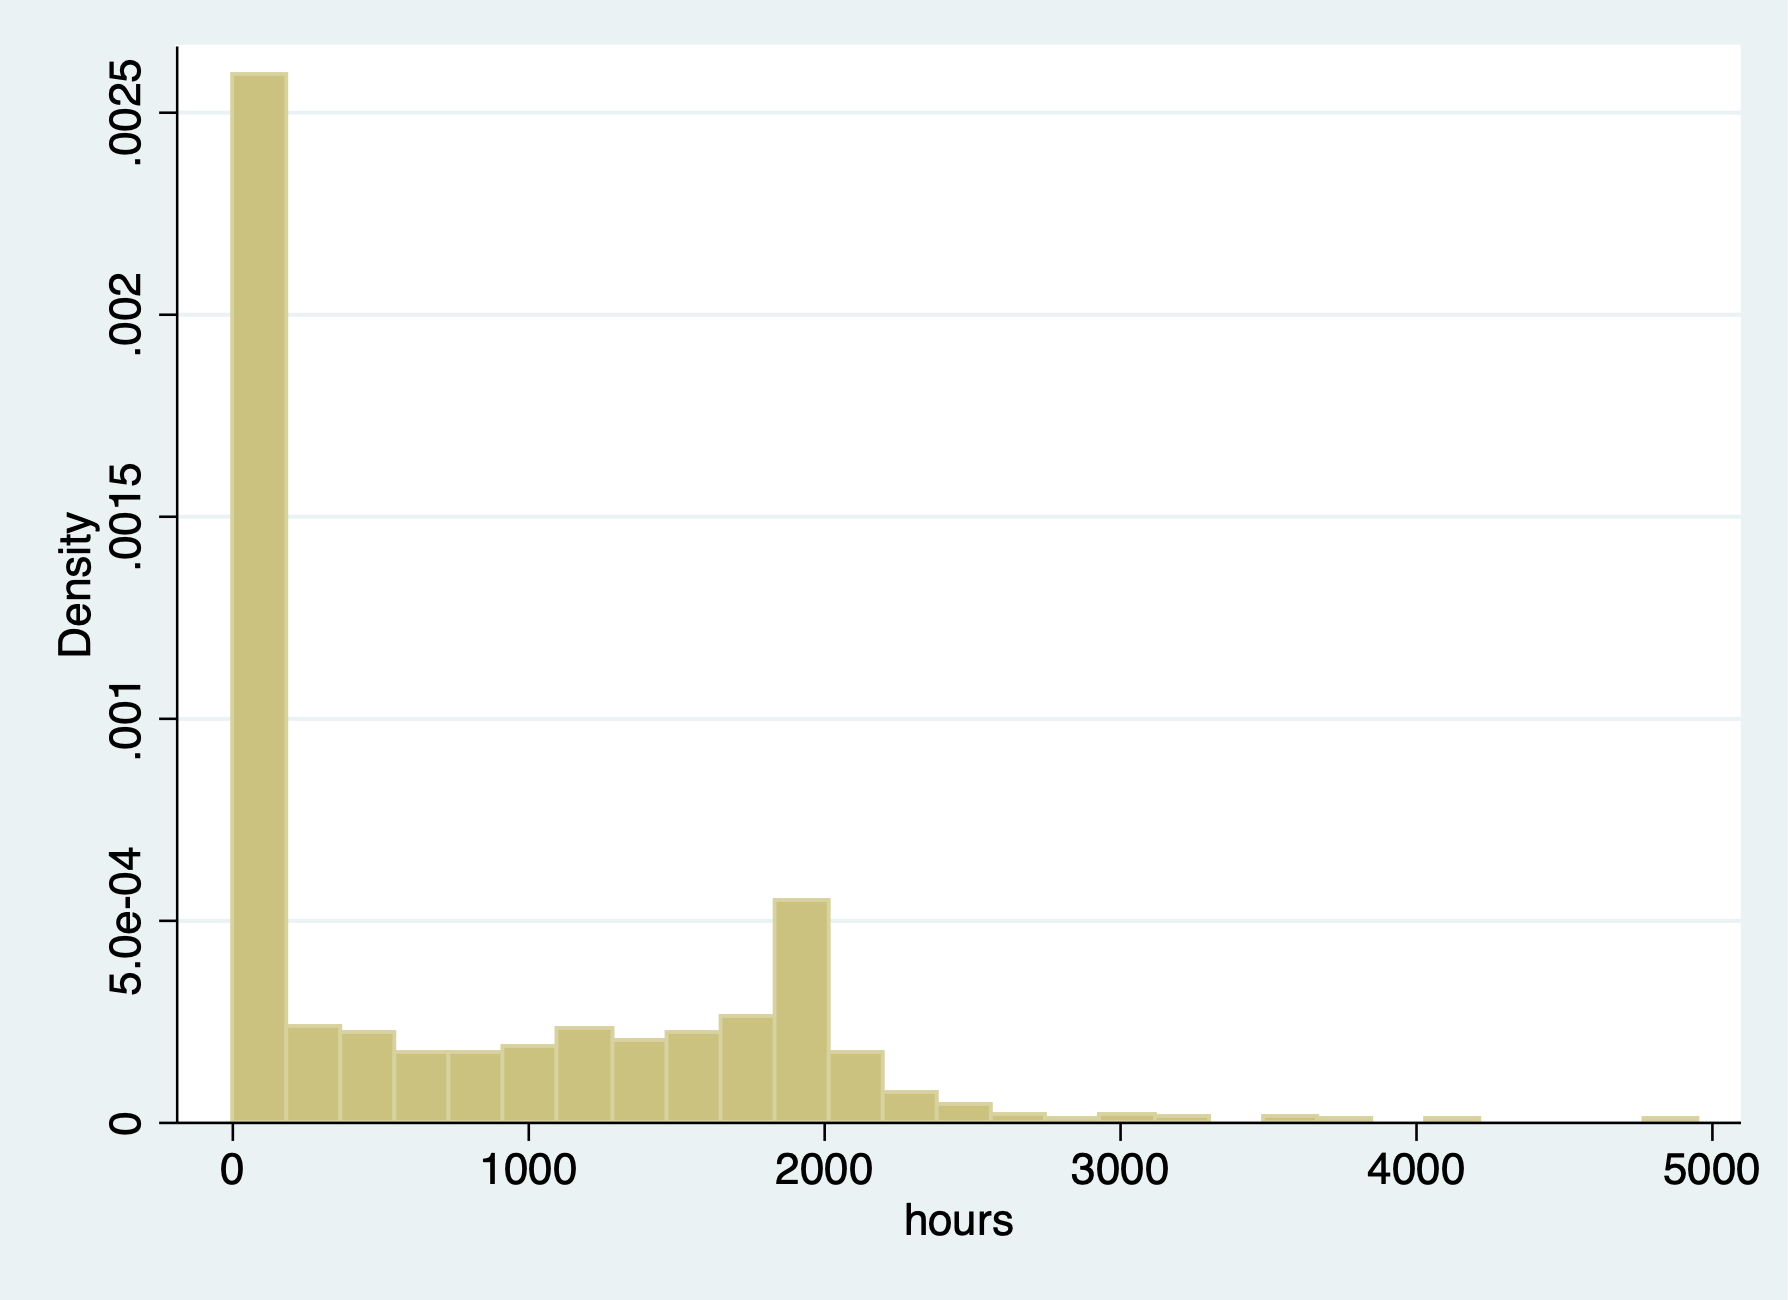
\includegraphics[keepaspectratio]{week8_hourhist.png}}
We have corner solution for women have 0 hours of labor

The range for women who do have working hours - ranges from 12 to 4950 hours

\begin{Shaded}
\begin{Highlighting}[]
\KeywordTok{sum}\NormalTok{ hours }\KeywordTok{if}\NormalTok{ hours \textgreater{} 0}
\end{Highlighting}
\end{Shaded}

\begin{verbatim}
    Variable |        Obs        Mean    Std. Dev.       Min        Max
-------------+---------------------------------------------------------
       hours |        428     1302.93    776.2744         12       4950
\end{verbatim}

\subsection*{OLS Model}\label{ols-model}
\addcontentsline{toc}{subsection}{OLS Model}

\begin{Shaded}
\begin{Highlighting}[]
\KeywordTok{est} \KeywordTok{clear}
\NormalTok{eststo OLS: }\KeywordTok{reg}\NormalTok{ hours nwifeinc educ exper expersq age kidslt6 kidsge6}
\NormalTok{margins}
\end{Highlighting}
\end{Shaded}

\begin{verbatim}
      Source |       SS           df       MS      Number of obs   =       753
-------------+----------------------------------   F(7, 745)       =     38.50
       Model |   151647606         7  21663943.7   Prob > F        =    0.0000
    Residual |   419262118       745  562767.944   R-squared       =    0.2656
-------------+----------------------------------   Adj R-squared   =    0.2587
       Total |   570909724       752  759188.463   Root MSE        =    750.18

------------------------------------------------------------------------------
       hours |      Coef.   Std. Err.      t    P>|t|     [95% Conf. Interval]
-------------+----------------------------------------------------------------
    nwifeinc |  -3.446636      2.544    -1.35   0.176    -8.440898    1.547626
        educ |   28.76112   12.95459     2.22   0.027     3.329283    54.19297
       exper |   65.67251   9.962983     6.59   0.000     46.11365    85.23138
     expersq |  -.7004939   .3245501    -2.16   0.031    -1.337635   -.0633524
         age |  -30.51163   4.363868    -6.99   0.000    -39.07858   -21.94469
     kidslt6 |  -442.0899    58.8466    -7.51   0.000    -557.6148    -326.565
     kidsge6 |  -32.77923   23.17622    -1.41   0.158     -78.2777    12.71924
       _cons |   1330.482   270.7846     4.91   0.000     798.8906    1862.074
------------------------------------------------------------------------------


Predictive margins                              Number of obs     =        753
Model VCE    : OLS

Expression   : Linear prediction, predict()

------------------------------------------------------------------------------
             |            Delta-method
             |     Margin   Std. Err.      t    P>|t|     [95% Conf. Interval]
-------------+----------------------------------------------------------------
       _cons |   740.5764   27.33803    27.09   0.000     686.9076    794.2451
------------------------------------------------------------------------------
\end{verbatim}

\subsection*{Tobit Model}\label{tobit-model}
\addcontentsline{toc}{subsection}{Tobit Model}

\begin{Shaded}
\begin{Highlighting}[]
\NormalTok{eststo TOBIT: }\KeywordTok{tobit}\NormalTok{ hours nwifeinc educ exper expersq age kidslt6 kidsge6, ll(0)}
\KeywordTok{quietly} \KeywordTok{sum}\NormalTok{ exper}
\KeywordTok{local}\NormalTok{ exp2=}\FunctionTok{r}\NormalTok{(}\KeywordTok{mean}\NormalTok{)\^{}2}
\end{Highlighting}
\end{Shaded}

\begin{verbatim}
Tobit regression                                Number of obs     =        753
                                                LR chi2(7)        =     271.59
                                                Prob > chi2       =     0.0000
Log likelihood = -3819.0946                     Pseudo R2         =     0.0343

------------------------------------------------------------------------------
       hours |      Coef.   Std. Err.      t    P>|t|     [95% Conf. Interval]
-------------+----------------------------------------------------------------
    nwifeinc |  -8.814243   4.459096    -1.98   0.048    -17.56811   -.0603724
        educ |   80.64561   21.58322     3.74   0.000     38.27453    123.0167
       exper |   131.5643   17.27938     7.61   0.000     97.64231    165.4863
     expersq |  -1.864158   .5376615    -3.47   0.001    -2.919667   -.8086479
         age |  -54.40501   7.418496    -7.33   0.000    -68.96862    -39.8414
     kidslt6 |  -894.0217   111.8779    -7.99   0.000    -1113.655   -674.3887
     kidsge6 |    -16.218   38.64136    -0.42   0.675    -92.07675    59.64075
       _cons |   965.3053   446.4358     2.16   0.031     88.88528    1841.725
-------------+----------------------------------------------------------------
      /sigma |   1122.022   41.57903                      1040.396    1203.647
------------------------------------------------------------------------------
           325  left-censored observations at hours <= 0
           428     uncensored observations
             0 right-censored observations
\end{verbatim}

\subsubsection*{Average Marginal Effects}\label{average-marginal-effects}
\addcontentsline{toc}{subsubsection}{Average Marginal Effects}

Using \emph{ystar} option with the \emph{margins} command tells Stata to act like there is no censoring even though the model allows for it
Statelist Discussion 1531196

\begin{Shaded}
\begin{Highlighting}[]
\KeywordTok{quietly}\NormalTok{ margins, }\KeywordTok{dydx}\NormalTok{(*) }\KeywordTok{predict}\NormalTok{(ystar(0,.)) }\FunctionTok{at}\NormalTok{(expersq=}\OtherTok{\textasciigrave{}exp2\textquotesingle{}}\NormalTok{)}
\NormalTok{eststo AME: margins, }\KeywordTok{dydx}\NormalTok{(*) }\KeywordTok{predict}\NormalTok{(ystar(0,.)) }\FunctionTok{at}\NormalTok{(expersq=}\OtherTok{\textasciigrave{}exp2\textquotesingle{}}\NormalTok{) }\KeywordTok{post}
\end{Highlighting}
\end{Shaded}

\begin{verbatim}
Average marginal effects                        Number of obs     =        753
Model VCE    : OIM

Expression   : E(hours*|hours>0), predict(ystar(0,.))
dy/dx w.r.t. : nwifeinc educ exper expersq age kidslt6 kidsge6
at           : expersq         =    113.0141

------------------------------------------------------------------------------
             |            Delta-method
             |      dy/dx   Std. Err.      z    P>|z|     [95% Conf. Interval]
-------------+----------------------------------------------------------------
    nwifeinc |  -5.223903   2.639553    -1.98   0.048    -10.39733   -.0504745
        educ |   47.79592    12.7368     3.75   0.000     22.83224     72.7596
       exper |    77.9737   9.900685     7.88   0.000     58.56872    97.37869
     expersq |  -1.104823    .316282    -3.49   0.000    -1.724724   -.4849218
         age |  -32.24401   4.348403    -7.42   0.000    -40.76672   -23.72129
     kidslt6 |  -529.8564   65.40462    -8.10   0.000    -658.0471   -401.6657
     kidsge6 |  -9.611857   22.90535    -0.42   0.675    -54.50553    35.28181
------------------------------------------------------------------------------
\end{verbatim}

Don't forget to use the \emph{post} option when using \emph{eststo}

\subsubsection*{Marginal Effects at the Average}\label{marginal-effects-at-the-average}
\addcontentsline{toc}{subsubsection}{Marginal Effects at the Average}

We will need to rerun the Tobit again to get our marginal effects at the average.

\begin{Shaded}
\begin{Highlighting}[]
\KeywordTok{quietly} \KeywordTok{tobit}\NormalTok{ hours nwifeinc educ exper expersq age kidslt6 kidsge6, ll(0)}
\NormalTok{eststo MEA: margins, }\KeywordTok{dydx}\NormalTok{(*) }\KeywordTok{predict}\NormalTok{(ystar(0,.)) }\FunctionTok{at}\NormalTok{(expersq=}\OtherTok{\textasciigrave{}exp2\textquotesingle{}}\NormalTok{) atmeans }\KeywordTok{post}
\end{Highlighting}
\end{Shaded}

\begin{verbatim}
Conditional marginal effects                    Number of obs     =        753
Model VCE    : OIM

Expression   : E(hours*|hours>0), predict(ystar(0,.))
dy/dx w.r.t. : nwifeinc educ exper expersq age kidslt6 kidsge6
at           : nwifeinc        =    20.12896 (mean)
               educ            =    12.28685 (mean)
               exper           =    10.63081 (mean)
               expersq         =    113.0141
               age             =    42.53785 (mean)
               kidslt6         =    .2377158 (mean)
               kidsge6         =    1.353254 (mean)

------------------------------------------------------------------------------
             |            Delta-method
             |      dy/dx   Std. Err.      z    P>|z|     [95% Conf. Interval]
-------------+----------------------------------------------------------------
    nwifeinc |  -5.687381   2.877882    -1.98   0.048    -11.32793   -.0468358
        educ |   52.03649   13.82013     3.77   0.000     24.94954    79.12345
       exper |   84.89173   12.39757     6.85   0.000     60.59293    109.1905
     expersq |  -1.202846   .3666136    -3.28   0.001    -1.921395   -.4842964
         age |  -35.10478   4.669466    -7.52   0.000    -44.25676   -25.95279
     kidslt6 |  -576.8666   70.92986    -8.13   0.000    -715.8866   -437.8466
     kidsge6 |  -10.46465   24.93972    -0.42   0.675    -59.34561    38.41632
------------------------------------------------------------------------------
\end{verbatim}

Compare our results. Remember we cannot directly OLS and Tobit due to the scale factor.

\begin{Shaded}
\begin{Highlighting}[]
\NormalTok{esttab OLS TOBIT, mtitle}
\end{Highlighting}
\end{Shaded}

\begin{verbatim}
                      (1)             (2)   
                      OLS           TOBIT   
--------------------------------------------
main                                        
nwifeinc           -3.447          -8.814*  
                  (-1.35)         (-1.98)   

educ                28.76*          80.65***
                   (2.22)          (3.74)   

exper               65.67***        131.6***
                   (6.59)          (7.61)   

expersq            -0.700*         -1.864***
                  (-2.16)         (-3.47)   

age                -30.51***       -54.41***
                  (-6.99)         (-7.33)   

kidslt6            -442.1***       -894.0***
                  (-7.51)         (-7.99)   

kidsge6            -32.78          -16.22   
                  (-1.41)         (-0.42)   

_cons              1330.5***        965.3*  
                   (4.91)          (2.16)   
--------------------------------------------
sigma                                       
_cons                              1122.0***
                                  (26.99)   
--------------------------------------------
N                     753             753   
--------------------------------------------
t statistics in parentheses
* p<0.05, ** p<0.01, *** p<0.001
\end{verbatim}

Compare OLS and Average Marginal Effects and Marginal Effects at the Average.

\begin{Shaded}
\begin{Highlighting}[]
\NormalTok{esttab OLS AME MEA, mtitle(}\StringTok{"OLS"} \StringTok{"AME"} \StringTok{"MEA"}\NormalTok{)}
\end{Highlighting}
\end{Shaded}

\begin{verbatim}
                      (1)             (2)             (3)   
                      OLS             AME             MEA   
------------------------------------------------------------
nwifeinc           -3.447          -5.224*         -5.687*  
                  (-1.35)         (-1.98)         (-1.98)   

educ                28.76*          47.80***        52.04***
                   (2.22)          (3.75)          (3.77)   

exper               65.67***        77.97***        84.89***
                   (6.59)          (7.88)          (6.85)   

expersq            -0.700*         -1.105***       -1.203** 
                  (-2.16)         (-3.49)         (-3.28)   

age                -30.51***       -32.24***       -35.10***
                  (-6.99)         (-7.42)         (-7.52)   

kidslt6            -442.1***       -529.9***       -576.9***
                  (-7.51)         (-8.10)         (-8.13)   

kidsge6            -32.78          -9.612          -10.46   
                  (-1.41)         (-0.42)         (-0.42)   

_cons              1330.5***                                
                   (4.91)                                   
------------------------------------------------------------
N                     753             753             753   
------------------------------------------------------------
t statistics in parentheses
* p<0.05, ** p<0.01, *** p<0.001
\end{verbatim}

When we compare marginal effects, we see that an additional year of education increases annual hours by 48 to 52 hours with the Tobit estimator. We see that an additional child less than 6 reduces the annual hours by a range of 530 to 577 hours.

\subsection*{Graph Results}\label{graph-results}
\addcontentsline{toc}{subsection}{Graph Results}

\begin{Shaded}
\begin{Highlighting}[]
\KeywordTok{est} \KeywordTok{clear}
\end{Highlighting}
\end{Shaded}

\subsubsection*{OLS Model}\label{ols-model-1}
\addcontentsline{toc}{subsubsection}{OLS Model}

\begin{Shaded}
\begin{Highlighting}[]
\KeywordTok{quietly} \KeywordTok{reg}\NormalTok{ hours nwifeinc educ exper expersq age kidslt6 kidsge6}
\NormalTok{eststo OLS: }\KeywordTok{quietly}\NormalTok{ margins, }\FunctionTok{at}\NormalTok{(educ=(0(2)20)) }\KeywordTok{post}
\end{Highlighting}
\end{Shaded}

\subsubsection*{Tobit Model}\label{tobit-model-1}
\addcontentsline{toc}{subsubsection}{Tobit Model}

\begin{Shaded}
\begin{Highlighting}[]
\KeywordTok{quietly} \KeywordTok{tobit}\NormalTok{ hours nwifeinc educ exper expersq age kidslt6 kidsge6, ll(0)}
\NormalTok{eststo Tobit: }\KeywordTok{quietly}\NormalTok{ margins, }\FunctionTok{at}\NormalTok{(educ=(0(2)20)) }\KeywordTok{predict}\NormalTok{(}\FunctionTok{e}\NormalTok{(0,6000)) }\KeywordTok{post}
\end{Highlighting}
\end{Shaded}

\subsubsection*{Coefplot}\label{coefplot}
\addcontentsline{toc}{subsubsection}{Coefplot}

\begin{Shaded}
\begin{Highlighting}[]
\NormalTok{coefplot (OLS, ciopts(}\KeywordTok{recast}\NormalTok{(rline) lpattern(solid))) (Tobit, ciopts(}\KeywordTok{recast}\NormalTok{(rline) lpattern(}\KeywordTok{dash}\NormalTok{))), }\FunctionTok{at} \KeywordTok{recast}\NormalTok{(}\KeywordTok{line}\NormalTok{)}

\KeywordTok{graph} \KeywordTok{export} \StringTok{"/Users/Sam/Desktop/Econ 645/Stata/week8\_tobitols.png"}\NormalTok{, }\KeywordTok{replace}
\end{Highlighting}
\end{Shaded}

\begin{figure}
\centering
\pandocbounded{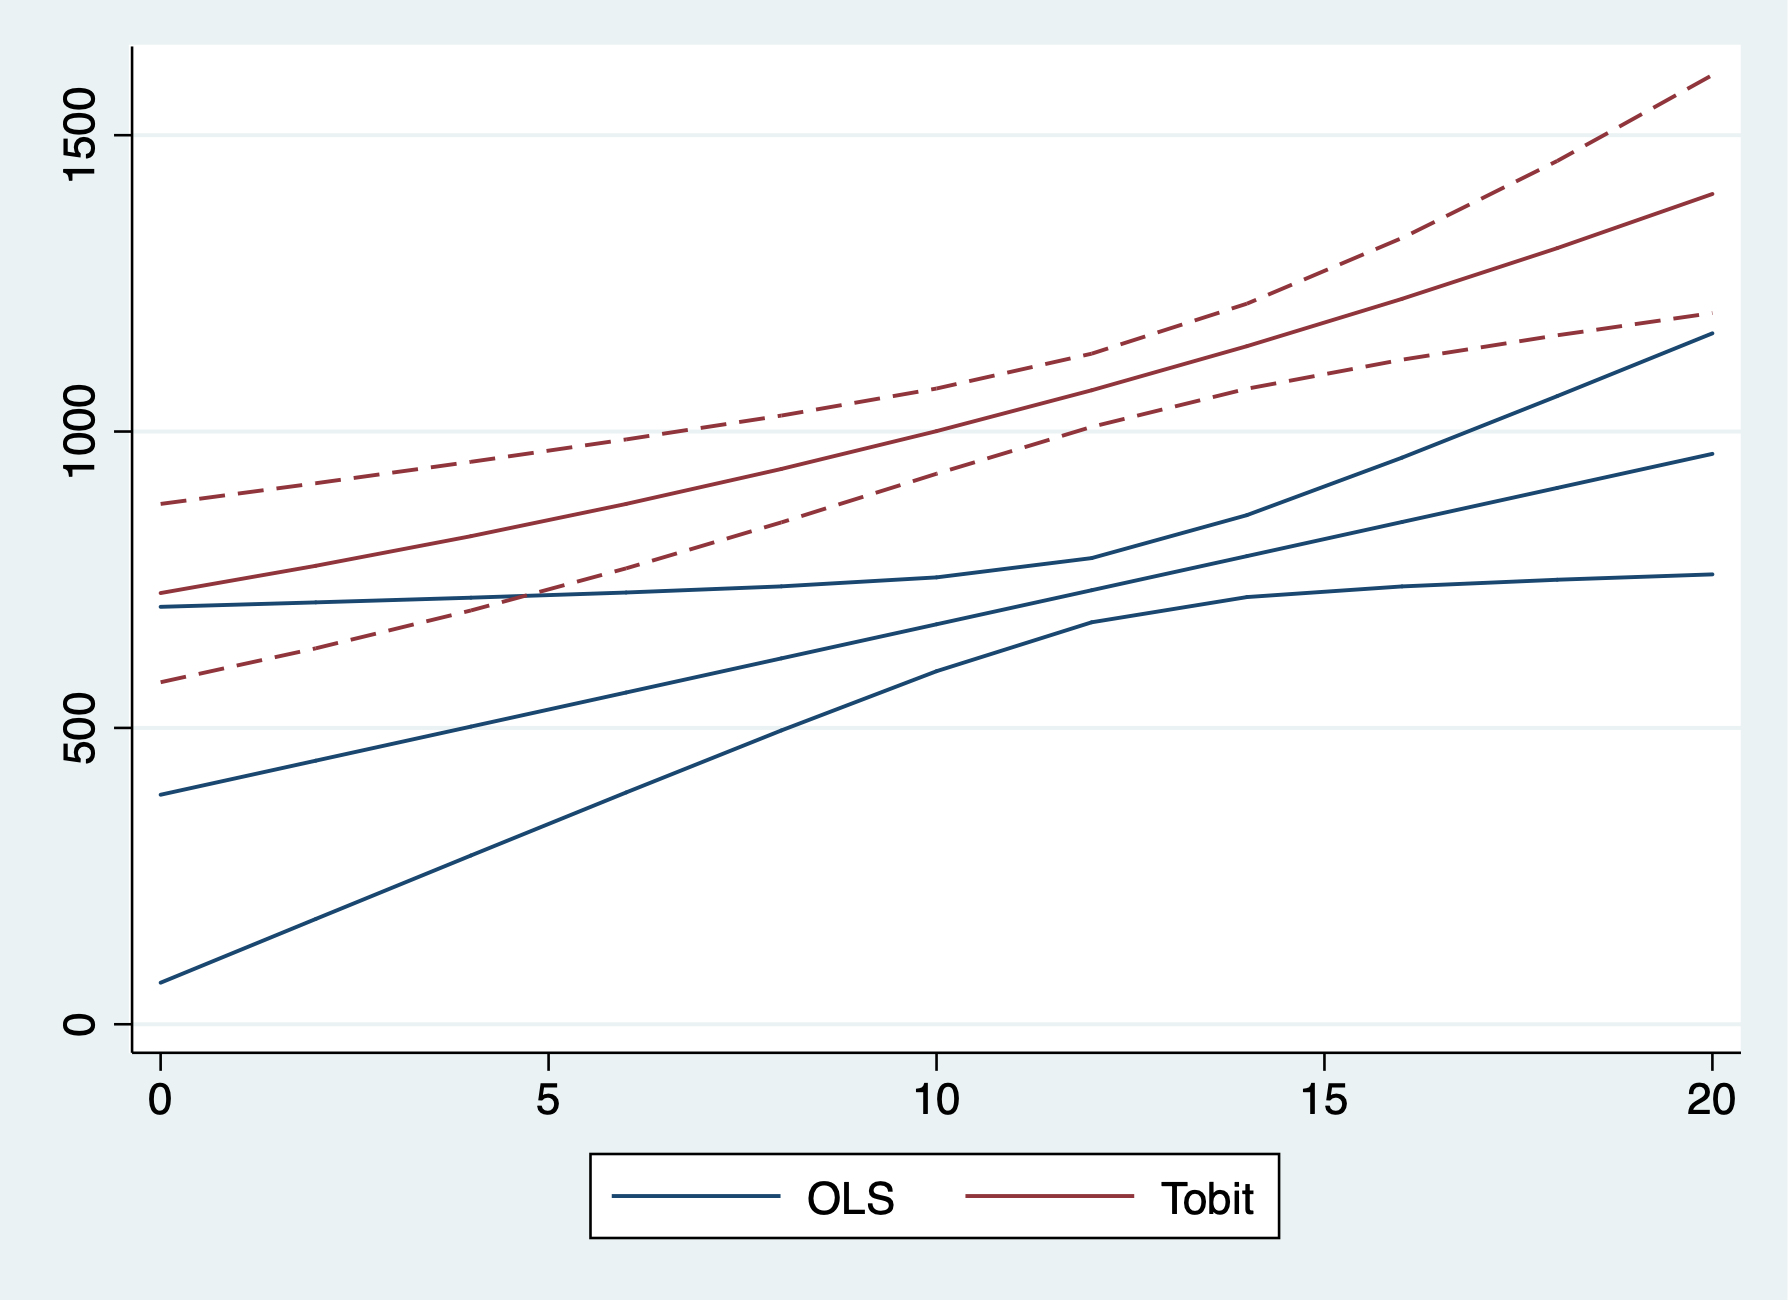
\includegraphics[keepaspectratio]{week8_tobitols.png}}
\caption{OLS vs Tobit Coefficients}
\end{figure}

\chapter{Poisson Regression}\label{poisson-regression}

\textbf{Lesson:} We should use a count model when we have a Poisson distribution for the outcome of interest. Our coefficients are expected log counts so we *need to transform our coefficients for interpretation.

We want to look at arrest data to see the number of times a man was arrested in 1986. There are 1,970 zeros out of 2,725 men in the sample and only eight observations are greater than 5. An OLS will not account for a count model but a Poisson distribution will.

We have
1. pcnv - proportion of prior arrest that lead to a conviction
2. avgsen - the average sentence served from prior convictions (in months)
3. tottime - months spent in prison since age 18 prior to 1986
4. ptime86 - months spent in prison in 1986
5. qemp86 - number of quarters that the person was legally employed in 1986
6. inc86 - income in 1986
7. Hispanic - Hispanic/Latino binary
8. Black - Black binary
9. ptime86 - prison time in 1986

\[ narr86_{t}=\alpha + \beta_1 pcnv_t + \beta_2 avgsen_t + \beta_3 tottime_t + \beta_4 ptime86_t + \beta_5 qemp86_t + \beta_6 inc86_t + x'_t\delta + \varepsilon_t  \]

\subsection*{OLS}\label{ols}
\addcontentsline{toc}{subsection}{OLS}

\begin{Shaded}
\begin{Highlighting}[]
\NormalTok{cd }\StringTok{"/Users/Sam/Desktop/Econ 645/Data/Wooldridge"}
\KeywordTok{use} \StringTok{"crime1.dta"}\NormalTok{, }\KeywordTok{clear}
\KeywordTok{reg}\NormalTok{ narr86 pcnv avgsen tottime ptime86 qemp86 inc86 }\BaseNTok{black}\NormalTok{ hispan born60 }
\end{Highlighting}
\end{Shaded}

\begin{verbatim}
/Users/Sam/Desktop/Econ 645/Data/Wooldridge

      Source |       SS           df       MS      Number of obs   =     2,725
-------------+----------------------------------   F(9, 2715)      =     23.57
       Model |  145.702778         9  16.1891976   Prob > F        =    0.0000
    Residual |  1864.64438     2,715  .686793509   R-squared       =    0.0725
-------------+----------------------------------   Adj R-squared   =    0.0694
       Total |  2010.34716     2,724  .738012906   Root MSE        =    .82873

------------------------------------------------------------------------------
      narr86 |      Coef.   Std. Err.      t    P>|t|     [95% Conf. Interval]
-------------+----------------------------------------------------------------
        pcnv |   -.131886   .0404037    -3.26   0.001    -.2111112   -.0526609
      avgsen |  -.0113316   .0122413    -0.93   0.355    -.0353348    .0126717
     tottime |   .0120693   .0094364     1.28   0.201     -.006434    .0305725
     ptime86 |  -.0408735    .008813    -4.64   0.000    -.0581544   -.0235925
      qemp86 |  -.0513099   .0144862    -3.54   0.000     -.079715   -.0229047
       inc86 |  -.0014617    .000343    -4.26   0.000    -.0021343   -.0007891
       black |   .3270097   .0454264     7.20   0.000     .2379359    .4160835
      hispan |   .1938094   .0397156     4.88   0.000     .1159335    .2716853
      born60 |   -.022465   .0332945    -0.67   0.500    -.0877502    .0428202
       _cons |    .576566   .0378945    15.22   0.000      .502261    .6508711
------------------------------------------------------------------------------
\end{verbatim}

\subsection*{Poisson}\label{poisson}
\addcontentsline{toc}{subsection}{Poisson}

We use the \emph{poisson} command to estimate a Poisson regression. \textbf{Our coefficients are the change in expected log counts.} We will need a transformation to interpret the results.

\begin{Shaded}
\begin{Highlighting}[]
\KeywordTok{poisson}\NormalTok{ narr86 pcnv avgsen tottime ptime86 qemp86 inc86 }\BaseNTok{black}\NormalTok{ hispan born60 }
\end{Highlighting}
\end{Shaded}

\begin{verbatim}
Iteration 0:   log likelihood = -2249.0104  
Iteration 1:   log likelihood = -2248.7614  
Iteration 2:   log likelihood = -2248.7611  
Iteration 3:   log likelihood = -2248.7611  

Poisson regression                              Number of obs     =      2,725
                                                LR chi2(9)        =     386.32
                                                Prob > chi2       =     0.0000
Log likelihood = -2248.7611                     Pseudo R2         =     0.0791

------------------------------------------------------------------------------
      narr86 |      Coef.   Std. Err.      z    P>|z|     [95% Conf. Interval]
-------------+----------------------------------------------------------------
        pcnv |  -.4015713   .0849712    -4.73   0.000    -.5681117   -.2350308
      avgsen |  -.0237723    .019946    -1.19   0.233    -.0628658    .0153212
     tottime |   .0244904   .0147504     1.66   0.097    -.0044199    .0534006
     ptime86 |  -.0985584   .0206946    -4.76   0.000    -.1391192   -.0579977
      qemp86 |  -.0380187   .0290242    -1.31   0.190    -.0949051    .0188677
       inc86 |  -.0080807    .001041    -7.76   0.000     -.010121   -.0060404
       black |   .6608376   .0738342     8.95   0.000     .5161252      .80555
      hispan |   .4998133   .0739267     6.76   0.000     .3549196     .644707
      born60 |  -.0510286   .0640518    -0.80   0.426    -.1765678    .0745106
       _cons |  -.5995888   .0672501    -8.92   0.000    -.7313966    -.467781
------------------------------------------------------------------------------
\end{verbatim}

Test \(E(y|x)=Var(y|x)\)

\begin{Shaded}
\begin{Highlighting}[]
\KeywordTok{estat}\NormalTok{ gof}
\end{Highlighting}
\end{Shaded}

\begin{verbatim}
         Deviance goodness-of-fit =  2822.185
         Prob > chi2(2715)        =    0.0742

         Pearson goodness-of-fit  =   4118.08
         Prob > chi2(2715)        =    0.0000
\end{verbatim}

\subsubsection*{Factor Change Interpretation}\label{factor-change-interpretation}
\addcontentsline{toc}{subsubsection}{Factor Change Interpretation}

\(\Delta pcnv = .01\) so

\begin{Shaded}
\begin{Highlighting}[]
\KeywordTok{display}\NormalTok{ (}\FunctionTok{exp}\NormalTok{({-}.402*.01){-}1)*100}
\end{Highlighting}
\end{Shaded}

\begin{verbatim}
-.40119306
\end{verbatim}

A 1 percentage point increase in prior arrest decreases \textbf{expected number} of arrests by 0.4\%

A discrete change in a binary - the coefficient on Black

\begin{Shaded}
\begin{Highlighting}[]
\KeywordTok{display}\NormalTok{ (}\FunctionTok{exp}\NormalTok{(0.6608){-}1)*100 }
\end{Highlighting}
\end{Shaded}

\begin{verbatim}
93.634079
\end{verbatim}

This means that the \textbf{expected number} of arrests for a Black person is 93.7\% higher than the expected number of arrests for a White person.

We can use the command \emph{listcoef} as well, where \(e^{\beta}\) or \((e^{\beta}-1)*100\) depending upon the option called percent.

\begin{Shaded}
\begin{Highlighting}[]
\NormalTok{scc install listcoef}
\NormalTok{listcoef, }\KeywordTok{help}
\NormalTok{listcoef, }\KeywordTok{percent} \KeywordTok{help}
\end{Highlighting}
\end{Shaded}

\subsubsection*{Marginal Effects}\label{marginal-effects}
\addcontentsline{toc}{subsubsection}{Marginal Effects}

\textbf{Interpretation:} The marginal change in a continuous variable depends on the expected value of \(y\)
given \(x\), so we have to calculate marginal effects by specifing x at their means or calculate average marginal effects.

\textbf{Note:} be careful with the change in percentage points for pcnv, we want a 1 percentage or 10 percentage point change not a change of 1 (or 100 percentage points)

\begin{Shaded}
\begin{Highlighting}[]
\NormalTok{margins, }\KeywordTok{dydx}\NormalTok{(*)}
\end{Highlighting}
\end{Shaded}

\begin{verbatim}
Average marginal effects                        Number of obs     =      2,725
Model VCE    : OIM

Expression   : Predicted number of events, predict()
dy/dx w.r.t. : pcnv avgsen tottime ptime86 qemp86 inc86 black hispan born60

------------------------------------------------------------------------------
             |            Delta-method
             |      dy/dx   Std. Err.      z    P>|z|     [95% Conf. Interval]
-------------+----------------------------------------------------------------
        pcnv |  -.1623969   .0347091    -4.68   0.000    -.2304256   -.0943682
      avgsen |  -.0096136   .0080714    -1.19   0.234    -.0254333    .0062061
     tottime |    .009904   .0059726     1.66   0.097     -.001802      .02161
     ptime86 |  -.0398574   .0084547    -4.71   0.000    -.0564283   -.0232865
      qemp86 |  -.0153749   .0117466    -1.31   0.191    -.0383979    .0076481
       inc86 |  -.0032679   .0004323    -7.56   0.000    -.0041152   -.0024205
       black |   .2672451   .0309251     8.64   0.000     .2066331    .3278571
      hispan |   .2021263     .03051     6.62   0.000     .1423279    .2619248
      born60 |  -.0206361   .0259102    -0.80   0.426    -.0714193     .030147
------------------------------------------------------------------------------
\end{verbatim}

\subsubsection*{Incident-Rate Ratios}\label{incident-rate-ratios}
\addcontentsline{toc}{subsubsection}{Incident-Rate Ratios}

\begin{Shaded}
\begin{Highlighting}[]
\KeywordTok{poisson}\NormalTok{ narr86 pcnv avgsen tottime ptime86 qemp86 inc86 }\BaseNTok{black}\NormalTok{ hispan born60, }\KeywordTok{irr}
\end{Highlighting}
\end{Shaded}

\begin{verbatim}
Iteration 0:   log likelihood = -2249.0104  
Iteration 1:   log likelihood = -2248.7614  
Iteration 2:   log likelihood = -2248.7611  
Iteration 3:   log likelihood = -2248.7611  

Poisson regression                              Number of obs     =      2,725
                                                LR chi2(9)        =     386.32
                                                Prob > chi2       =     0.0000
Log likelihood = -2248.7611                     Pseudo R2         =     0.0791

------------------------------------------------------------------------------
      narr86 |        IRR   Std. Err.      z    P>|z|     [95% Conf. Interval]
-------------+----------------------------------------------------------------
        pcnv |   .6692676   .0568685    -4.73   0.000     .5665943    .7905465
      avgsen |    .976508   .0194775    -1.19   0.233     .9390695    1.015439
     tottime |   1.024793   .0151161     1.66   0.097     .9955899    1.054852
     ptime86 |   .9061427   .0187523    -4.76   0.000     .8701243    .9436521
      qemp86 |   .9626949   .0279415    -1.31   0.190     .9094592    1.019047
       inc86 |   .9919519   .0010326    -7.76   0.000       .98993    .9939778
       black |   1.936414   .1429736     8.95   0.000     1.675523    2.237927
      hispan |   1.648413   .1218618     6.76   0.000     1.426066    1.905429
      born60 |   .9502515   .0608653    -0.80   0.426     .8381419    1.077357
       _cons |   .5490374   .0369228    -8.92   0.000     .4812364    .6263907
------------------------------------------------------------------------------
\end{verbatim}

\chapter{Negative Binomial Regression Model}\label{negative-binomial-regression-model}

\textbf{Lesson: When overdispersion occurs, we could estimate a Negative Binomial Regression model. We'll see that our standard errors might be too large if our main Poisson assumption mean=variance fails.}

\subsection*{Poisson}\label{poisson-1}
\addcontentsline{toc}{subsection}{Poisson}

First, we will estimate a poisson regression.

\begin{Shaded}
\begin{Highlighting}[]
\NormalTok{cd }\StringTok{"/Users/Sam/Desktop/Econ 645/Data/Wooldridge"}
\KeywordTok{use} \StringTok{"crime1.dta"}\NormalTok{, }\KeywordTok{clear}
\KeywordTok{est} \KeywordTok{clear}
\NormalTok{eststo PRM: }\KeywordTok{poisson}\NormalTok{ narr86 pcnv avgsen tottime ptime86 qemp86 inc86 }\BaseNTok{black}\NormalTok{ hispan born60 }
\end{Highlighting}
\end{Shaded}

\subsection*{Negative Binomial}\label{negative-binomial}
\addcontentsline{toc}{subsection}{Negative Binomial}

We use the \emph{nbreg} command to estimate a negative binomial regression.

\begin{Shaded}
\begin{Highlighting}[]
\NormalTok{eststo NBRM: }\KeywordTok{nbreg}\NormalTok{ narr86 pcnv avgsen tottime ptime86 qemp86 inc86 }\BaseNTok{black}\NormalTok{ hispan born60 }
\end{Highlighting}
\end{Shaded}

\begin{verbatim}
Fitting Poisson model:

Iteration 0:   log likelihood = -2249.0104  
Iteration 1:   log likelihood = -2248.7614  
Iteration 2:   log likelihood = -2248.7611  
Iteration 3:   log likelihood = -2248.7611  

Fitting constant-only model:

Iteration 0:   log likelihood = -2297.3847  
Iteration 1:   log likelihood = -2291.4767  
Iteration 2:   log likelihood = -2290.6926  
Iteration 3:   log likelihood = -2290.6903  
Iteration 4:   log likelihood = -2290.6903  

Fitting full model:

Iteration 0:   log likelihood = -2181.2355  
Iteration 1:   log likelihood = -2158.2716  
Iteration 2:   log likelihood = -2157.6284  
Iteration 3:   log likelihood =  -2157.628  
Iteration 4:   log likelihood =  -2157.628  

Negative binomial regression                    Number of obs     =      2,725
                                                LR chi2(9)        =     266.12
Dispersion     = mean                           Prob > chi2       =     0.0000
Log likelihood =  -2157.628                     Pseudo R2         =     0.0581

------------------------------------------------------------------------------
      narr86 |      Coef.   Std. Err.      z    P>|z|     [95% Conf. Interval]
-------------+----------------------------------------------------------------
        pcnv |  -.4770963   .1033295    -4.62   0.000    -.6796183   -.2745743
      avgsen |  -.0173385   .0261171    -0.66   0.507    -.0685272    .0338501
     tottime |   .0197394   .0192325     1.03   0.305    -.0179557    .0574344
     ptime86 |  -.1073997    .025074    -4.28   0.000    -.1565439   -.0582555
      qemp86 |  -.0504884   .0351857    -1.43   0.151    -.1194511    .0184743
       inc86 |  -.0077126   .0011465    -6.73   0.000    -.0099596   -.0054656
       black |   .6560406   .0923594     7.10   0.000     .4750195    .8370617
      hispan |   .5048465   .0895663     5.64   0.000     .3292998    .6803932
      born60 |   -.046412   .0776384    -0.60   0.550    -.1985804    .1057564
       _cons |  -.5637368   .0827121    -6.82   0.000    -.7258495   -.4016242
-------------+----------------------------------------------------------------
    /lnalpha |  -.0738912   .1177617                     -.3046999    .1569175
-------------+----------------------------------------------------------------
       alpha |   .9287728   .1093739                      .7373446    1.169899
------------------------------------------------------------------------------
LR test of alpha=0: chibar2(01) = 182.27               Prob >= chibar2 = 0.000
\end{verbatim}

First, our coefficients are the change in \textbf{expected log counts}, so we need some transformations
to provide interpretations.

Second, our test for over dispersion can be seen at the bottom of our NBRM output with the LR test of \(\alpha = 0\)

\subsubsection*{Factor Change}\label{factor-change}
\addcontentsline{toc}{subsubsection}{Factor Change}

We can manually calculate \(e^{\beta}\) to interpret the results with a factor change, or we can use the \emph{listcoef} command:

\begin{Shaded}
\begin{Highlighting}[]
\NormalTok{listcoef, }\KeywordTok{percent} \KeywordTok{help}
\NormalTok{listcoef, }\KeywordTok{help}
\end{Highlighting}
\end{Shaded}

\begin{verbatim}
nbreg (N=2725): Percentage Change in Expected Count 

 Observed SD: .85907678

------------------------------------------------------------------
  narr86 |      b         z     P>|z|      %      %StdX      SDofX
---------+--------------------------------------------------------
    pcnv |  -0.47710   -4.617   0.000    -37.9    -17.2     0.3952
  avgsen |  -0.01734   -0.664   0.507     -1.7     -5.9     3.5080
 tottime |   0.01974    1.026   0.305      2.0      9.5     4.6070
 ptime86 |  -0.10740   -4.283   0.000    -10.2    -18.9     1.9501
  qemp86 |  -0.05049   -1.435   0.151     -4.9     -7.8     1.6104
   inc86 |  -0.00771   -6.727   0.000     -0.8    -40.2    66.6272
   black |   0.65604    7.103   0.000     92.7     27.3     0.3677
  hispan |   0.50485    5.637   0.000     65.7     23.2     0.4127
  born60 |  -0.04641   -0.598   0.550     -4.5     -2.2     0.4808
---------+--------------------------------------------------------
ln alpha |  -0.07389   -0.627
------------------------------------------------------------------
       b = raw coefficient
       z = z-score for test of b=0
   P>|z| = p-value for z-test
       % = percent change in expected count for unit increase in X
   %StdX = percent change in expected count for SD increase in X
   SDofX = standard deviation of X


nbreg (N=2725): Factor Change in Expected Count 

 Observed SD: .85907678

------------------------------------------------------------------
  narr86 |      b         z     P>|z|    e^b    e^bStdX      SDofX
---------+--------------------------------------------------------
    pcnv |  -0.47710   -4.617   0.000   0.6206   0.8282     0.3952
  avgsen |  -0.01734   -0.664   0.507   0.9828   0.9410     3.5080
 tottime |   0.01974    1.026   0.305   1.0199   1.0952     4.6070
 ptime86 |  -0.10740   -4.283   0.000   0.8982   0.8110     1.9501
  qemp86 |  -0.05049   -1.435   0.151   0.9508   0.9219     1.6104
   inc86 |  -0.00771   -6.727   0.000   0.9923   0.5982    66.6272
   black |   0.65604    7.103   0.000   1.9271   1.2728     0.3677
  hispan |   0.50485    5.637   0.000   1.6567   1.2316     0.4127
  born60 |  -0.04641   -0.598   0.550   0.9546   0.9779     0.4808
---------+--------------------------------------------------------
ln alpha |  -0.07389   -0.627
------------------------------------------------------------------
       b = raw coefficient
       z = z-score for test of b=0
   P>|z| = p-value for z-test
     e^b = exp(b) = factor change in expected count for unit increase in X
 e^bStdX = exp(b*SD of X) = change in expected count for SD increase in X
   SDofX = standard deviation of X
\end{verbatim}

Let's look at pcnv:

\begin{Shaded}
\begin{Highlighting}[]
\KeywordTok{display} \FunctionTok{exp}\NormalTok{({-}.4771*.1){-}1}
\end{Highlighting}
\end{Shaded}

\begin{verbatim}
-.04658976
\end{verbatim}

A 10 percentage point increase in proportion of prior arrests that lead to conviction decrease the expected number of arrests by 4.7\% holding all others constant.

Let's look at avgsen:

\begin{Shaded}
\begin{Highlighting}[]
\KeywordTok{display}\NormalTok{ (}\FunctionTok{exp}\NormalTok{(0.01974){-}1)}
\end{Highlighting}
\end{Shaded}

\begin{verbatim}
.01993612
\end{verbatim}

a 1 month increase in total time served in prision from prior convictions before 1986 increases the expected number of arrests holding all others constant.

\begin{Shaded}
\begin{Highlighting}[]
\NormalTok{esttab, mtitle}
\end{Highlighting}
\end{Shaded}

\begin{verbatim}
                      (1)             (2)   
                      PRM            NBRM   
--------------------------------------------
narr86                                      
pcnv               -0.402***       -0.477***
                  (-4.73)         (-4.62)   

avgsen            -0.0238         -0.0173   
                  (-1.19)         (-0.66)   

tottime            0.0245          0.0197   
                   (1.66)          (1.03)   

ptime86           -0.0986***       -0.107***
                  (-4.76)         (-4.28)   

qemp86            -0.0380         -0.0505   
                  (-1.31)         (-1.43)   

inc86            -0.00808***     -0.00771***
                  (-7.76)         (-6.73)   

black               0.661***        0.656***
                   (8.95)          (7.10)   

hispan              0.500***        0.505***
                   (6.76)          (5.64)   

born60            -0.0510         -0.0464   
                  (-0.80)         (-0.60)   

_cons              -0.600***       -0.564***
                  (-8.92)         (-6.82)   
--------------------------------------------
lnalpha                                     
_cons                             -0.0739   
                                  (-0.63)   
--------------------------------------------
N                    2725            2725   
--------------------------------------------
t statistics in parentheses
* p<0.05, ** p<0.01, *** p<0.001
\end{verbatim}

\subsubsection*{Marginal Effects}\label{marginal-effects-1}
\addcontentsline{toc}{subsubsection}{Marginal Effects}

Interpretation is similar to Poisson
The marginal change in a continuous variable depends on the expected value of y
given x, so we have to specify x with atmeans or average marginal effects

\begin{Shaded}
\begin{Highlighting}[]
\NormalTok{margins, }\KeywordTok{dydx}\NormalTok{(*)}
\end{Highlighting}
\end{Shaded}

\begin{verbatim}
Average marginal effects                        Number of obs     =      2,725
Model VCE    : OIM

Expression   : Predicted number of events, predict()
dy/dx w.r.t. : pcnv avgsen tottime ptime86 qemp86 inc86 black hispan born60

------------------------------------------------------------------------------
             |            Delta-method
             |      dy/dx   Std. Err.      z    P>|z|     [95% Conf. Interval]
-------------+----------------------------------------------------------------
        pcnv |  -.1933482   .0429858    -4.50   0.000    -.2775988   -.1090976
      avgsen |  -.0070266    .010587    -0.66   0.507    -.0277767    .0137235
     tottime |   .0079996   .0078006     1.03   0.305    -.0072894    .0232886
     ptime86 |  -.0435248   .0103794    -4.19   0.000    -.0638682   -.0231815
      qemp86 |  -.0204609   .0143136    -1.43   0.153    -.0485151    .0075932
       inc86 |  -.0031256   .0004821    -6.48   0.000    -.0040705   -.0021807
       black |   .2658672   .0395274     6.73   0.000     .1883949    .3433395
      hispan |   .2045942   .0375363     5.45   0.000     .1310244    .2781641
      born60 |  -.0188089   .0314753    -0.60   0.550    -.0804994    .0428815
------------------------------------------------------------------------------
\end{verbatim}

\subsubsection*{Incident Rate Ratios}\label{incident-rate-ratios-1}
\addcontentsline{toc}{subsubsection}{Incident Rate Ratios}

We can also use the option \emph{irr} to calcualte incident-rate ratios.

\begin{Shaded}
\begin{Highlighting}[]
\KeywordTok{nbreg}\NormalTok{ narr86 pcnv avgsen tottime ptime86 qemp86 inc86 }\BaseNTok{black}\NormalTok{ hispan born60, }\KeywordTok{irr}
\end{Highlighting}
\end{Shaded}

\begin{verbatim}
Fitting Poisson model:

Iteration 0:   log likelihood = -2249.0104  
Iteration 1:   log likelihood = -2248.7614  
Iteration 2:   log likelihood = -2248.7611  
Iteration 3:   log likelihood = -2248.7611  

Fitting constant-only model:

Iteration 0:   log likelihood = -2297.3847  
Iteration 1:   log likelihood = -2291.4767  
Iteration 2:   log likelihood = -2290.6926  
Iteration 3:   log likelihood = -2290.6903  
Iteration 4:   log likelihood = -2290.6903  

Fitting full model:

Iteration 0:   log likelihood = -2181.2355  
Iteration 1:   log likelihood = -2158.2716  
Iteration 2:   log likelihood = -2157.6284  
Iteration 3:   log likelihood =  -2157.628  
Iteration 4:   log likelihood =  -2157.628  

Negative binomial regression                    Number of obs     =      2,725
                                                LR chi2(9)        =     266.12
Dispersion     = mean                           Prob > chi2       =     0.0000
Log likelihood =  -2157.628                     Pseudo R2         =     0.0581

------------------------------------------------------------------------------
      narr86 |        IRR   Std. Err.      z    P>|z|     [95% Conf. Interval]
-------------+----------------------------------------------------------------
        pcnv |   .6205828   .0641245    -4.62   0.000     .5068104    .7598956
      avgsen |   .9828109   .0256682    -0.66   0.507     .9337681     1.03443
     tottime |   1.019935   .0196159     1.03   0.305     .9822046    1.059116
     ptime86 |   .8981666   .0225207    -4.28   0.000     .8550939    .9434089
      qemp86 |    .950765   .0334533    -1.43   0.151     .8874074    1.018646
       inc86 |   .9923171   .0011377    -6.73   0.000     .9900898    .9945493
       black |   1.927147   .1779901     7.10   0.000     1.608046    2.309571
      hispan |   1.656731   .1483873     5.64   0.000     1.389994    1.974654
      born60 |   .9546486   .0741174    -0.60   0.550     .8198939    1.111551
       _cons |   .5690785   .0470697    -6.82   0.000     .4839133    .6692322
-------------+----------------------------------------------------------------
    /lnalpha |  -.0738912   .1177617                     -.3046999    .1569175
-------------+----------------------------------------------------------------
       alpha |   .9287728   .1093739                      .7373446    1.169899
------------------------------------------------------------------------------
LR test of alpha=0: chibar2(01) = 182.27               Prob >= chibar2 = 0.000
\end{verbatim}

\chapter{Processing observations across subgroups}\label{processing-observations-across-subgroups}

One thing Stata easily provides are commands and options for subgroup
analysis. We can use the by prefix command to create and analyze subgroups
or cross-sectional units in a panel data set.

\section{Obtaining separate results for subgroups}\label{obtaining-separate-results-for-subgroups}

\emph{Tabulate} is a very helpful command to analyze categorical variables, or occassionally look through continuous variables (as long as there aren't too many values).

The \emph{tabulate} command has an option to summarize a continuous variable when tabulating categorical variables.

\begin{Shaded}
\begin{Highlighting}[]
\NormalTok{cd }\StringTok{"/Users/Sam/Desktop/Econ 645/Data/Mitchell"}
\KeywordTok{use}\NormalTok{ wws2, }\KeywordTok{clear}
\KeywordTok{tabulate}\NormalTok{ married, }\KeywordTok{summarize}\NormalTok{(wage)}
\end{Highlighting}
\end{Shaded}

\begin{verbatim}
/Users/Sam/Desktop/Econ 645/Data/Mitchell

(Working Women Survey w/fixes)

            |       Summary of hourly wage
    married |        Mean   Std. Dev.       Freq.
------------+------------------------------------
          0 |   8.0920006    6.354849         804
          1 |   7.6319496   5.5017864       1,440
------------+------------------------------------
      Total |   7.7967807   5.8245895       2,244
\end{verbatim}

Another option is using the bysort prefix command.

\begin{Shaded}
\begin{Highlighting}[]
\KeywordTok{bysort}\NormalTok{ married: }\KeywordTok{summarize}\NormalTok{ wage}
\end{Highlighting}
\end{Shaded}

\begin{verbatim}
-> married = 0

    Variable |        Obs        Mean    Std. Dev.       Min        Max
-------------+---------------------------------------------------------
        wage |        804    8.092001    6.354849          0   40.19808

------------------------------------------------------------------------------------------------------------------
-> married = 1

    Variable |        Obs        Mean    Std. Dev.       Min        Max
-------------+---------------------------------------------------------
        wage |      1,440     7.63195    5.501786   1.004952   40.74659
\end{verbatim}

We can also correlate data within groups instead of using qualifiers and additional statements.

With qualifiers

\begin{Shaded}
\begin{Highlighting}[]
\NormalTok{correlate wage age }\KeywordTok{if}\NormalTok{ married == 0}
\NormalTok{correlate wage age }\KeywordTok{if}\NormalTok{ married == 1}
\end{Highlighting}
\end{Shaded}

\begin{verbatim}
(obs=804)

             |     wage      age
-------------+------------------
        wage |   1.0000
         age |  -0.0185   1.0000


(obs=1,440)

             |     wage      age
-------------+------------------
        wage |   1.0000
         age |   0.0049   1.0000
\end{verbatim}

Using bysort accomplishes this in one command

\begin{Shaded}
\begin{Highlighting}[]
\KeywordTok{bysort}\NormalTok{ married: correlate wage age}
\end{Highlighting}
\end{Shaded}

\begin{verbatim}
-> married = 0
(obs=804)

             |     wage      age
-------------+------------------
        wage |   1.0000
         age |  -0.0185   1.0000


------------------------------------------------------------------------------------------------------------------
-> married = 1
(obs=1,440)

             |     wage      age
-------------+------------------
        wage |   1.0000
         age |   0.0049   1.0000
\end{verbatim}

Using bysort accomplishes even faster if we have a categorical variable with many categories

\begin{Shaded}
\begin{Highlighting}[]
\KeywordTok{bysort}\NormalTok{ race: correlate wage age}
\end{Highlighting}
\end{Shaded}

\begin{verbatim}
-> race = 1
(obs=1,637)

             |     wage      age
-------------+------------------
        wage |   1.0000
         age |   0.0017   1.0000


------------------------------------------------------------------------------------------------------------------
-> race = 2
(obs=581)

             |     wage      age
-------------+------------------
        wage |   1.0000
         age |  -0.0331   1.0000


------------------------------------------------------------------------------------------------------------------
-> race = 3
(obs=26)

             |     wage      age
-------------+------------------
        wage |   1.0000
         age |  -0.2194   1.0000
\end{verbatim}

\section{Computing values separately by subgroups}\label{computing-values-separately-by-subgroups}

The by prefix command and the \emph{egen} command is a powerful combination that
makes aggregating group statistics much easier than other statistical
software packages

\emph{Bysort} and \emph{egen} makes aggregating by groups much easier than other software. R has aggregate which is flexible and powerful, but requires more coding compared to \emph{egen}.

I'm not the biggest fan of Mitchell's examples with \emph{bysort var: egen}, but they get the job done. I would like us to use some CPS examples with \emph{bysort} and \emph{egen}.

With bysort var: egen we can calculate subgroup statistics, counts, summations
with one easy line of code

\begin{Shaded}
\begin{Highlighting}[]
\NormalTok{cd }\StringTok{"/Users/Sam/Desktop/Econ 645/Data/Mitchell"}
\KeywordTok{use}\NormalTok{ tv1, }\KeywordTok{clear}
\OtherTok{list}\NormalTok{, sepby(kidid)}
\end{Highlighting}
\end{Shaded}

\begin{verbatim}
/Users/Sam/Desktop/Econ 645/Data/Mitchell

     +--------------------------------------------+
     | kidid          dt   female   wt   tv   vac |
     |--------------------------------------------|
  1. |     1   07jan2002        1   53    1     1 |
  2. |     1   08jan2002        1   55    3     1 |
     |--------------------------------------------|
  3. |     2   16jan2002        1   58    8     1 |
     |--------------------------------------------|
  4. |     3   18jan2002        0   60    2     0 |
  5. |     3   19jan2002        0   63    5     1 |
  6. |     3   21jan2002        0   66    1     1 |
  7. |     3   22jan2002        0   64    6     0 |
     |--------------------------------------------|
  8. |     4   10jan2002        1   62    7     0 |
  9. |     4   11jan2002        1   58    1     0 |
 10. |     4   13jan2002        1   55    4     0 |
     +--------------------------------------------+
\end{verbatim}

If we want to calculate the average tv time for each kid we first sort by
the child id and then use egen. We may have multiple levels and we can use
bysort to find the multiple level identifiers such as id, year, and month of year.

\begin{Shaded}
\begin{Highlighting}[]
\KeywordTok{bysort}\NormalTok{ kidid: }\KeywordTok{egen}\NormalTok{ avgtv = }\KeywordTok{mean}\NormalTok{(tv)}
\KeywordTok{sort}\NormalTok{ kidid}
\OtherTok{list}\NormalTok{ kidid tv avgtv, sepby(kidid)}
\end{Highlighting}
\end{Shaded}

\begin{verbatim}
     | kidid   tv   avgtv |
     |--------------------|
  1. |     1    1       2 |
  2. |     1    3       2 |
     |--------------------|
  3. |     2    8       8 |
     |--------------------|
  4. |     3    2     3.5 |
  5. |     3    5     3.5 |
  6. |     3    1     3.5 |
  7. |     3    6     3.5 |
     |--------------------|
  8. |     4    7       4 |
  9. |     4    1       4 |
 10. |     4    4       4 |
     +--------------------+
\end{verbatim}

If we want the standard deviation of the child's tv watching.Let's generate some z-scores and look at the statistics.

\begin{Shaded}
\begin{Highlighting}[]
\KeywordTok{bysort}\NormalTok{ kidid: }\KeywordTok{egen}\NormalTok{ sdtv = }\FunctionTok{sd}\NormalTok{(tv)}
\KeywordTok{generate}\NormalTok{ ztv = (tv{-}avgtv)/sdtv}
\OtherTok{list} 
\end{Highlighting}
\end{Shaded}

\begin{verbatim}
(1 missing value generated)

(1 missing value generated)

     +-----------------------------------------------------------------------------+
     | kidid          dt   female   wt   tv   vac   avgtv        sdtv          ztv |
     |-----------------------------------------------------------------------------|
  1. |     1   07jan2002        1   53    1     1       2   1.4142136   -.70710678 |
  2. |     1   08jan2002        1   55    3     1       2   1.4142136    .70710678 |
  3. |     2   16jan2002        1   58    8     1       8           .            . |
  4. |     3   18jan2002        0   60    2     0     3.5   2.3804761   -.63012604 |
  5. |     3   19jan2002        0   63    5     1     3.5   2.3804761    .63012604 |
     |-----------------------------------------------------------------------------|
  6. |     3   21jan2002        0   66    1     1     3.5   2.3804761   -1.0502101 |
  7. |     3   22jan2002        0   64    6     0     3.5   2.3804761    1.0502101 |
  8. |     4   10jan2002        1   62    7     0       4           3            1 |
  9. |     4   11jan2002        1   58    1     0       4           3           -1 |
 10. |     4   13jan2002        1   55    4     0       4           3            0 |
     +-----------------------------------------------------------------------------+
\end{verbatim}

Let's generate some subgroup statistics for a binary variable vac.
Where vac=0 if the kid was not on vacation and vac=1 if the kid was on vacation.

\begin{Shaded}
\begin{Highlighting}[]
\KeywordTok{bysort}\NormalTok{ kidid: }\KeywordTok{egen}\NormalTok{ vac\_total = }\KeywordTok{total}\NormalTok{(vac)}
\KeywordTok{bysort}\NormalTok{ kidid: }\KeywordTok{egen}\NormalTok{ vac\_sd = }\FunctionTok{sd}\NormalTok{(vac)}
\KeywordTok{bysort}\NormalTok{ kidid: }\KeywordTok{egen}\NormalTok{ vac\_min = }\FunctionTok{min}\NormalTok{(vac)}
\KeywordTok{bysort}\NormalTok{ kidid: }\KeywordTok{egen}\NormalTok{ vac\_max = }\FunctionTok{max}\NormalTok{(vac)}
\OtherTok{list}\NormalTok{ kidid vac*, sepby(kidid) abb(10)}
\end{Highlighting}
\end{Shaded}

\begin{verbatim}
(1 missing value generated)

     +---------------------------------------------------------+
     | kidid   vac   vac_total      vac_sd   vac_min   vac_max |
     |---------------------------------------------------------|
  1. |     1     1           2           0         1         1 |
  2. |     1     1           2           0         1         1 |
     |---------------------------------------------------------|
  3. |     2     1           1           .         1         1 |
     |---------------------------------------------------------|
  4. |     3     0           2   .57735027         0         1 |
  5. |     3     1           2   .57735027         0         1 |
  6. |     3     1           2   .57735027         0         1 |
  7. |     3     0           2   .57735027         0         1 |
     |---------------------------------------------------------|
  8. |     4     0           0           0         0         0 |
  9. |     4     0           0           0         0         0 |
 10. |     4     0           0           0         0         0 |
     +---------------------------------------------------------+
\end{verbatim}

Let's see if some kids watch less than 4 hours of tv per day.
We'll generate a binary/dummy variable to be 1 if equal to or less than 4 hours
a day and 0 if it is greater than 4 hours a day.

\begin{Shaded}
\begin{Highlighting}[]
\KeywordTok{generate}\NormalTok{ tvlo = (tv \textless{} 4) }\KeywordTok{if}\NormalTok{ !}\FunctionTok{missing}\NormalTok{(tv)}
\end{Highlighting}
\end{Shaded}

We can generate individual level subgroup analysis with bysort and egen on
binary variables

\begin{Shaded}
\begin{Highlighting}[]
\KeywordTok{bysort}\NormalTok{ kidid: }\KeywordTok{egen}\NormalTok{ tvlocnt = }\FunctionTok{count}\NormalTok{(tvlo)}
\KeywordTok{bysort}\NormalTok{ kidid: }\KeywordTok{egen}\NormalTok{ tvlototal = }\KeywordTok{total}\NormalTok{(tvlo)}
\KeywordTok{bysort}\NormalTok{ kidid: }\KeywordTok{egen}\NormalTok{ tvlosum = }\KeywordTok{sum}\NormalTok{(tvlo)}
\KeywordTok{bysort}\NormalTok{ kidid: }\KeywordTok{gen}\NormalTok{ tvlosum2 = }\KeywordTok{sum}\NormalTok{(tvlo)}
\KeywordTok{bysort}\NormalTok{ kidid: }\KeywordTok{egen}\NormalTok{ tvlosame = }\FunctionTok{sd}\NormalTok{(tvlo)}
\KeywordTok{bysort}\NormalTok{ kidid: }\KeywordTok{egen}\NormalTok{ tvloall = }\FunctionTok{min}\NormalTok{(tvlo)}
\KeywordTok{bysort}\NormalTok{ kidid: }\KeywordTok{egen}\NormalTok{ tvloever = }\FunctionTok{max}\NormalTok{(tvlo)}
\OtherTok{list}\NormalTok{ kidid tv tvlo*, sepby(kidid) abb(20)}
\end{Highlighting}
\end{Shaded}

\begin{verbatim}
(1 missing value generated)

     +-----------------------------------------------------------------------------------------------+
     | kidid   tv   tvlo   tvlocnt   tvlototal   tvlosum   tvlosum2    tvlosame   tvloall   tvloever |
     |-----------------------------------------------------------------------------------------------|
  1. |     1    1      1         2           2         2          1           0         1          1 |
  2. |     1    3      1         2           2         2          2           0         1          1 |
     |-----------------------------------------------------------------------------------------------|
  3. |     2    8      0         1           0         0          0           .         0          0 |
     |-----------------------------------------------------------------------------------------------|
  4. |     3    2      1         4           2         2          1   .57735027         0          1 |
  5. |     3    5      0         4           2         2          1   .57735027         0          1 |
  6. |     3    1      1         4           2         2          2   .57735027         0          1 |
  7. |     3    6      0         4           2         2          2   .57735027         0          1 |
     |-----------------------------------------------------------------------------------------------|
  8. |     4    7      0         3           1         1          0   .57735027         0          1 |
  9. |     4    1      1         3           1         1          1   .57735027         0          1 |
 10. |     4    4      0         3           1         1          1   .57735027         0          1 |
     +-----------------------------------------------------------------------------------------------+
\end{verbatim}

Notice how \emph{count()} provides the number of observations for each kid, while
\emph{total()} returns a constant for the sum of all values, but so does \emph{egen sum()}.
The problem is that there is a \emph{gen var = sum(var2)} function that returns
a \textbf{running sum} that we see in tvsum2. Use \emph{egen sum} with caution if you want a cumulative sum. If you want a cumulative sum use \emph{egen total()}.

We have our central tendencies functions with

\begin{enumerate}
\def\labelenumi{\arabic{enumi}.}
\tightlist
\item
  \emph{mean()},
\item
  \emph{median()},
\item
  \emph{mode()}.
\end{enumerate}

We can find percentiles with

\begin{enumerate}
\def\labelenumi{\arabic{enumi}.}
\tightlist
\item
  \emph{pctile(var), p(\#)}.
\end{enumerate}

We have other \emph{egen} functions that may be of help, such as

\begin{enumerate}
\def\labelenumi{\arabic{enumi}.}
\tightlist
\item
  Interquartile Range \emph{iqr()},
\item
  Median Absolute Deviation \emph{mad()},
\item
  Mean Absolute Deviation \emph{mdev()},
\item
  Kurtosis \emph{kurt()}
\item
  Skewness \emph{skew()}.
\item
  Other functions
\end{enumerate}

\begin{Shaded}
\begin{Highlighting}[]
\KeywordTok{help} \KeywordTok{egen}
\end{Highlighting}
\end{Shaded}

Mitchell has a good note here:

\emph{Egen mean()} takes an arguement, not a varlist, so if you put
\emph{bysort idvar: egen meanvars1\_5=mean(var1-var5)}, \emph{mean()} will return not the
means of vars 1 through 5, but var1 minus var5.

\section{Subscripting or Indexing: Computing values within subgroups:}\label{subscripting-or-indexing-computing-values-within-subgroups}

Unsolicated Opinion Alert:
Subscripting (or I may accidently call it indexing) is a very powerful tool
that I personally think puts Stata as the top paid statistical software
(I do think that R is more powerful and more flexible, but Stata balances
power, flexibility, and ease of learning).

Each variable is a vector x1=x{[}x11, x12, x13,\ldots,x1N{]} for i=1,\ldots,N observations
We can use a subscript or index to call which part of the vector we want to
return.

\begin{Shaded}
\begin{Highlighting}[]
\NormalTok{cd }\StringTok{"/Users/Sam/Desktop/Econ 645/Data/Mitchell"}
\KeywordTok{use}\NormalTok{ tv1, }\KeywordTok{clear}
\OtherTok{list}\NormalTok{, sepby(kidid)}
\end{Highlighting}
\end{Shaded}

\begin{verbatim}
/Users/Sam/Desktop/Econ 645/Data/Mitchell

     +--------------------------------------------+
     | kidid          dt   female   wt   tv   vac |
     |--------------------------------------------|
  1. |     1   07jan2002        1   53    1     1 |
  2. |     1   08jan2002        1   55    3     1 |
     |--------------------------------------------|
  3. |     2   16jan2002        1   58    8     1 |
     |--------------------------------------------|
  4. |     3   18jan2002        0   60    2     0 |
  5. |     3   19jan2002        0   63    5     1 |
  6. |     3   21jan2002        0   66    1     1 |
  7. |     3   22jan2002        0   64    6     0 |
     |--------------------------------------------|
  8. |     4   10jan2002        1   62    7     0 |
  9. |     4   11jan2002        1   58    1     0 |
 10. |     4   13jan2002        1   55    4     0 |
     +--------------------------------------------+
\end{verbatim}

If we want the first observation in our tv vector we can call it with {[}1{]}

\begin{Shaded}
\begin{Highlighting}[]
\KeywordTok{display}\NormalTok{ tv[1]}
\end{Highlighting}
\end{Shaded}

\begin{verbatim}
1
\end{verbatim}

We can look at the first kid id and date and time

\begin{Shaded}
\begin{Highlighting}[]
\KeywordTok{display} \StringTok{"kid: "}\NormalTok{ kidid[1] }\StringTok{", Date: "}\NormalTok{ dt[1] }\StringTok{", Sex: "}\NormalTok{ female[1] }\StringTok{", TV Hours: "}\NormalTok{ tv[1]}
\end{Highlighting}
\end{Shaded}

\begin{verbatim}
kid: 1, Date: 15347, Sex: 1, TV Hours: 1
\end{verbatim}

We can see the second observation

\begin{Shaded}
\begin{Highlighting}[]
\KeywordTok{display}\NormalTok{ tv[2]}
\end{Highlighting}
\end{Shaded}

\begin{verbatim}
3
\end{verbatim}

We can see the difference between the two observations

\begin{Shaded}
\begin{Highlighting}[]
\KeywordTok{display}\NormalTok{ tv[2]{-}tv[1]}
\end{Highlighting}
\end{Shaded}

\begin{verbatim}
2
\end{verbatim}

\textbf{Note:} we have some very useful system variables of \_N and \_n
\_N is total number of observations and when used in the subscript/index
it will return the last observation

\_n is current number of observations or observation number and when used in
the subscript/index it will return the current observation (almost like i=i+1)

\begin{Shaded}
\begin{Highlighting}[]
\KeywordTok{help}\NormalTok{ system variables}
\end{Highlighting}
\end{Shaded}

Subscripting is very helpful when working Panel Data. You can index within
cross-sectional units over time with ease. The subscript (or index) will
return the nth observation given

If we want the first observation to be compared to all observations

\begin{Shaded}
\begin{Highlighting}[]
\NormalTok{cd }\StringTok{"/Users/Sam/Desktop/Econ 645/Data/Mitchell"}
\KeywordTok{use}\NormalTok{ tv1, }\KeywordTok{clear}
\KeywordTok{bysort}\NormalTok{ kidid: }\KeywordTok{gen}\NormalTok{ tv\_1ob = tv[1]}
\OtherTok{list}\NormalTok{ kidid tv tv\_1ob, sepby(kidid)}
\end{Highlighting}
\end{Shaded}

\begin{verbatim}
/Users/Sam/Desktop/Econ 645/Data/Mitchell

     +---------------------+
     | kidid   tv   tv_1ob |
     |---------------------|
  1. |     1    1        1 |
  2. |     1    3        1 |
     |---------------------|
  3. |     2    8        8 |
     |---------------------|
  4. |     3    2        2 |
  5. |     3    5        2 |
  6. |     3    1        2 |
  7. |     3    6        2 |
     |---------------------|
  8. |     4    7        7 |
  9. |     4    1        7 |
 10. |     4    4        7 |
     +---------------------+
\end{verbatim}

If we want to compare the last observation to all observations

\begin{Shaded}
\begin{Highlighting}[]
\KeywordTok{bysort}\NormalTok{ kidid: }\KeywordTok{gen}\NormalTok{ tv\_lastob = tv[\_N]}
\OtherTok{list}\NormalTok{ kidid tv tv\_lastob, sepby(kidid)}
\end{Highlighting}
\end{Shaded}

\begin{verbatim}
     | kidid   tv   tv_las~b |
     |-----------------------|
  1. |     1    1          3 |
  2. |     1    3          3 |
     |-----------------------|
  3. |     2    8          8 |
     |-----------------------|
  4. |     3    2          6 |
  5. |     3    5          6 |
  6. |     3    1          6 |
  7. |     3    6          6 |
     |-----------------------|
  8. |     4    7          4 |
  9. |     4    1          4 |
 10. |     4    4          4 |
     +-----------------------+
\end{verbatim}

If we want the second to last observation

\begin{Shaded}
\begin{Highlighting}[]
\KeywordTok{bysort}\NormalTok{ kidid: }\KeywordTok{gen}\NormalTok{ tv\_2tolastob = tv[\_N{-}1]}
\OtherTok{list}\NormalTok{ kidid tv tv\_2tolastob, sepby(kidid)}
\end{Highlighting}
\end{Shaded}

\begin{verbatim}
(1 missing value generated)

     +-----------------------+
     | kidid   tv   tv_2to~b |
     |-----------------------|
  1. |     1    1          1 |
  2. |     1    3          1 |
     |-----------------------|
  3. |     2    8          . |
     |-----------------------|
  4. |     3    2          1 |
  5. |     3    5          1 |
  6. |     3    1          1 |
  7. |     3    6          1 |
     |-----------------------|
  8. |     4    7          1 |
  9. |     4    1          1 |
 10. |     4    4          1 |
     +-----------------------+
\end{verbatim}

If we want the prior observation (lag of 1)

\begin{Shaded}
\begin{Highlighting}[]
\KeywordTok{bysort}\NormalTok{ kidid: }\KeywordTok{gen}\NormalTok{ tv\_lagob = tv[}\DataTypeTok{\_n}\NormalTok{{-}1]}
\OtherTok{list}\NormalTok{ kidid tv tv\_lagob, sepby(kidid)}
\end{Highlighting}
\end{Shaded}

\begin{verbatim}
(4 missing values generated)

     +-----------------------+
     | kidid   tv   tv_lagob |
     |-----------------------|
  1. |     1    1          . |
  2. |     1    3          1 |
     |-----------------------|
  3. |     2    8          . |
     |-----------------------|
  4. |     3    2          . |
  5. |     3    5          2 |
  6. |     3    1          5 |
  7. |     3    6          1 |
     |-----------------------|
  8. |     4    7          . |
  9. |     4    1          7 |
 10. |     4    4          1 |
     +-----------------------+
\end{verbatim}

If we want the next observation (lead of 1)

\begin{Shaded}
\begin{Highlighting}[]
\KeywordTok{bysort}\NormalTok{ kidid: }\KeywordTok{gen}\NormalTok{ tv\_leadob = tv[}\DataTypeTok{\_n}\NormalTok{+1]}
\OtherTok{list}\NormalTok{ kidid tv tv\_leadob, sepby(kidid)}
\end{Highlighting}
\end{Shaded}

\begin{verbatim}
(4 missing values generated)

     +-----------------------+
     | kidid   tv   tv_lea~b |
     |-----------------------|
  1. |     1    1          3 |
  2. |     1    3          . |
     |-----------------------|
  3. |     2    8          . |
     |-----------------------|
  4. |     3    2          5 |
  5. |     3    5          1 |
  6. |     3    1          6 |
  7. |     3    6          . |
     |-----------------------|
  8. |     4    7          1 |
  9. |     4    1          4 |
 10. |     4    4          . |
     +-----------------------+
\end{verbatim}

You can use \emph{bysort kidid (dt)} to tell Stata to order by kid id and date,
but NOT INCLUDE dt in the grouping.

If we use kidid AND tv bysort kidid tv: egen, then we will look for observation
Within kid id AND the date. Since there is only 1 observation per kid
per date, we will only have 1 observation for each grouping.
If we want the first observation to be compared to all observations

\begin{Shaded}
\begin{Highlighting}[]
\NormalTok{cd }\StringTok{"/Users/Sam/Desktop/Econ 645/Data/Mitchell"}
\KeywordTok{use}\NormalTok{ tv1, }\KeywordTok{clear}
\KeywordTok{bysort}\NormalTok{ kidid (dt): }\KeywordTok{gen}\NormalTok{ tv\_1ob1 = tv[1]}
\KeywordTok{bysort}\NormalTok{ kidid dt: }\KeywordTok{gen}\NormalTok{ tv\_1ob2 = tv[1]}
\OtherTok{list}\NormalTok{ kidid tv tv\_1ob*, sepby(kidid)}
\end{Highlighting}
\end{Shaded}

\begin{verbatim}
/Users/Sam/Desktop/Econ 645/Data/Mitchell

     +--------------------------------+
     | kidid   tv   tv_1ob1   tv_1ob2 |
     |--------------------------------|
  1. |     1    1         1         1 |
  2. |     1    3         1         3 |
     |--------------------------------|
  3. |     2    8         8         8 |
     |--------------------------------|
  4. |     3    2         2         2 |
  5. |     3    5         2         5 |
  6. |     3    1         2         1 |
  7. |     3    6         2         6 |
     |--------------------------------|
  8. |     4    7         7         7 |
  9. |     4    1         7         1 |
 10. |     4    4         7         4 |
     +--------------------------------+
\end{verbatim}

If we want to compare the last observation to all observations

\begin{Shaded}
\begin{Highlighting}[]
\KeywordTok{bysort}\NormalTok{ kidid (dt): }\KeywordTok{gen}\NormalTok{ tv\_lastob1 = tv[\_N]}
\KeywordTok{bysort}\NormalTok{ kidid dt: }\KeywordTok{gen}\NormalTok{ tv\_lastob2 = tv[\_N]}
\OtherTok{list}\NormalTok{ kidid tv tv\_lastob*, sepby(kidid)}
\end{Highlighting}
\end{Shaded}

\begin{verbatim}
     | kidid   tv   tv_las~1   tv_las~2 |
     |----------------------------------|
  1. |     1    1          3          1 |
  2. |     1    3          3          3 |
     |----------------------------------|
  3. |     2    8          8          8 |
     |----------------------------------|
  4. |     3    2          6          2 |
  5. |     3    5          6          5 |
  6. |     3    1          6          1 |
  7. |     3    6          6          6 |
     |----------------------------------|
  8. |     4    7          4          7 |
  9. |     4    1          4          1 |
 10. |     4    4          4          4 |
     +----------------------------------+
\end{verbatim}

If we want the prior observation (lag of 1)

\begin{Shaded}
\begin{Highlighting}[]
\KeywordTok{bysort}\NormalTok{ kidid (dt): }\KeywordTok{gen}\NormalTok{ tv\_lagob1 = tv[}\DataTypeTok{\_n}\NormalTok{{-}1]}
\KeywordTok{bysort}\NormalTok{ kidid dt: }\KeywordTok{gen}\NormalTok{ tv\_lagob2 = tv[}\DataTypeTok{\_n}\NormalTok{{-}1]}
\OtherTok{list}\NormalTok{ kidid tv tv\_lagob*, sepby(kidid)}
\end{Highlighting}
\end{Shaded}

\begin{Shaded}
\begin{Highlighting}[]
\KeywordTok{quietly}\NormalTok{ \{}
\NormalTok{cd }\StringTok{"/Users/Sam/Desktop/Econ 645/Data/Mitchell"}
\KeywordTok{use}\NormalTok{ tv1, }\KeywordTok{clear}
\KeywordTok{bysort}\NormalTok{ kidid (dt): }\KeywordTok{gen}\NormalTok{ tv\_1ob1 = tv[1]}
\KeywordTok{bysort}\NormalTok{ kidid dt: }\KeywordTok{gen}\NormalTok{ tv\_1ob2 = tv[1]}
\KeywordTok{bysort}\NormalTok{ kidid (dt): }\KeywordTok{gen}\NormalTok{ tv\_lastob1 = tv[\_N]}
\KeywordTok{bysort}\NormalTok{ kidid dt: }\KeywordTok{gen}\NormalTok{ tv\_lastob2 = tv[\_N]}
\NormalTok{\}}
\KeywordTok{bysort}\NormalTok{ kidid (dt): }\KeywordTok{gen}\NormalTok{ tv\_lagob1 = tv[}\DataTypeTok{\_n}\NormalTok{{-}1]}
\KeywordTok{bysort}\NormalTok{ kidid dt: }\KeywordTok{gen}\NormalTok{ tv\_lagob2 = tv[}\DataTypeTok{\_n}\NormalTok{{-}1]}
\OtherTok{list}\NormalTok{ kidid tv tv\_lagob*, sepby(kidid)}
\end{Highlighting}
\end{Shaded}

\begin{verbatim}
(4 missing values generated)

(10 missing values generated)

     +----------------------------------+
     | kidid   tv   tv_lag~1   tv_lag~2 |
     |----------------------------------|
  1. |     1    1          .          . |
  2. |     1    3          1          . |
     |----------------------------------|
  3. |     2    8          .          . |
     |----------------------------------|
  4. |     3    2          .          . |
  5. |     3    5          2          . |
  6. |     3    1          5          . |
  7. |     3    6          1          . |
     |----------------------------------|
  8. |     4    7          .          . |
  9. |     4    1          7          . |
 10. |     4    4          1          . |
     +----------------------------------+
\end{verbatim}

\section{Computing values within subgroups: Computations across observations}\label{computing-values-within-subgroups-computations-across-observations}

Another powerful combination with subscripting/indexing is that we can the
generate command to create new variables that perform mathematical operators
on different observations WITHIN the vector

Difference in tv time between current period and prior period

\begin{Shaded}
\begin{Highlighting}[]
\NormalTok{cd }\StringTok{"/Users/Sam/Desktop/Econ 645/Data/Mitchell"}
\KeywordTok{use}\NormalTok{ tv1, }\KeywordTok{clear}
\KeywordTok{bysort}\NormalTok{ kidid (dt): }\KeywordTok{generate}\NormalTok{ tvdfp = tv {-} tv[}\DataTypeTok{\_n}\NormalTok{{-}1]}
\OtherTok{list}
\end{Highlighting}
\end{Shaded}

\begin{verbatim}
/Users/Sam/Desktop/Econ 645/Data/Mitchell


(4 missing values generated)

     +----------------------------------------------------+
     | kidid          dt   female   wt   tv   vac   tvdfp |
     |----------------------------------------------------|
  1. |     1   07jan2002        1   53    1     1       . |
  2. |     1   08jan2002        1   55    3     1       2 |
  3. |     2   16jan2002        1   58    8     1       . |
  4. |     3   18jan2002        0   60    2     0       . |
  5. |     3   19jan2002        0   63    5     1       3 |
     |----------------------------------------------------|
  6. |     3   21jan2002        0   66    1     1      -4 |
  7. |     3   22jan2002        0   64    6     0       5 |
  8. |     4   10jan2002        1   62    7     0       . |
  9. |     4   11jan2002        1   58    1     0      -6 |
 10. |     4   13jan2002        1   55    4     0       3 |
     +----------------------------------------------------+
\end{verbatim}

Difference in tv time between current period and next period

\begin{Shaded}
\begin{Highlighting}[]
\KeywordTok{bysort}\NormalTok{ kidid (dt): }\KeywordTok{generate}\NormalTok{ tvdfs = tv {-} tv[}\DataTypeTok{\_n}\NormalTok{+1]}
\end{Highlighting}
\end{Shaded}

Difference in tv time between current period and first period

\begin{Shaded}
\begin{Highlighting}[]
\KeywordTok{bysort}\NormalTok{ kidid (dt): }\KeywordTok{generate}\NormalTok{ tvdff = tv {-} tv[1]}
\end{Highlighting}
\end{Shaded}

Difference in tv time between current period and last period

\begin{Shaded}
\begin{Highlighting}[]
\KeywordTok{bysort}\NormalTok{ kidid (dt): }\KeywordTok{generate}\NormalTok{ tvdfl = tv {-} tv[\_N]}
\end{Highlighting}
\end{Shaded}

Difference between current period and 3-year moving average over time

\begin{Shaded}
\begin{Highlighting}[]
\KeywordTok{bysort}\NormalTok{ kidid (dt): }\KeywordTok{generate}\NormalTok{ tv3avg = (tv[}\DataTypeTok{\_n}\NormalTok{{-}1] + tv[}\DataTypeTok{\_n}\NormalTok{] + tv[}\DataTypeTok{\_n}\NormalTok{+1])/3}
\OtherTok{list}\NormalTok{ kidid dt tvd* tv3avg}
\end{Highlighting}
\end{Shaded}

\begin{verbatim}
(7 missing values generated)

     +---------------------------------------------------------------+
     | kidid          dt   tvdfp   tvdfs   tvdff   tvdfl      tv3avg |
     |---------------------------------------------------------------|
  1. |     1   07jan2002       .      -2       0      -2           . |
  2. |     1   08jan2002       2       .       2       0           . |
  3. |     2   16jan2002       .       .       0       0           . |
  4. |     3   18jan2002       .      -3       0      -4           . |
  5. |     3   19jan2002       3       4       3      -1   2.6666667 |
     |---------------------------------------------------------------|
  6. |     3   21jan2002      -4      -5      -1      -5           4 |
  7. |     3   22jan2002       5       .       4       0           . |
  8. |     4   10jan2002       .       6       0       3           . |
  9. |     4   11jan2002      -6      -3      -6      -3           4 |
 10. |     4   13jan2002       3       .      -3       0           . |
     +---------------------------------------------------------------+
\end{verbatim}

We can also rebase our vector. For example, we can rebase a deflator for the
period dollars we want.

\begin{Shaded}
\begin{Highlighting}[]
\NormalTok{cd }\StringTok{"/Users/Sam/Desktop/Econ 645/Data/Mitchell"}
\NormalTok{import excel }\KeywordTok{using} \StringTok{"cpi\_1993\_2023.xlsx"}\NormalTok{, cellrange(A12:P42) firstrow }\KeywordTok{clear}
\KeywordTok{keep}\NormalTok{ Year Annual}
\end{Highlighting}
\end{Shaded}

\begin{verbatim}
/Users/Sam/Desktop/Econ 645/Data/Mitchell
\end{verbatim}

Rebase in 1993 Dollars

\begin{Shaded}
\begin{Highlighting}[]
\KeywordTok{gen}\NormalTok{ rebase93 = Annual/Annual[1]*100}
\end{Highlighting}
\end{Shaded}

Rebase in 2022 Dollars

\begin{Shaded}
\begin{Highlighting}[]
\KeywordTok{gen}\NormalTok{ rebase22 = Annual/Annual[\_N]*100}
\end{Highlighting}
\end{Shaded}

Rebase to 2012

\begin{Shaded}
\begin{Highlighting}[]
\KeywordTok{gen}\NormalTok{ rebase12 = Annual/Annual[\_N{-}10]*100}
\OtherTok{list}
\end{Highlighting}
\end{Shaded}

\begin{verbatim}
     | Year    Annual    rebase93    rebase22    rebase12 |
     |----------------------------------------------------|
  1. | 1993     144.5         100   49.375545   62.937185 |
  2. | 1994     148.2   102.56055   50.639832   64.548725 |
  3. | 1995     152.4   105.46713   52.074969   66.378041 |
  4. | 1996     156.9   108.58131   53.612616   68.338023 |
  5. | 1997     160.5   111.07266   54.842733   69.906008 |
     |----------------------------------------------------|
  6. | 1998       163   112.80277   55.696981   70.994887 |
  7. | 1999     166.6   115.29412   56.927098   72.562872 |
  8. | 2000     172.2   119.16955   58.840614    75.00196 |
  9. | 2001     177.1   122.56055   60.514941   77.136162 |
 10. | 2002     179.9   124.49827   61.471699   78.355706 |
     |----------------------------------------------------|
 11. | 2003       184   127.33564   62.872666   80.141467 |
 12. | 2004     188.9   130.72664   64.546992   82.275669 |
 13. | 2005     195.3   135.15571   66.733868   85.063199 |
 14. | 2006     201.6   139.51557   68.886573   87.807173 |
 15. | 2007   207.342   143.48927    70.84861   90.308109 |
     |----------------------------------------------------|
 16. | 2008   215.303   148.99862   73.568878   93.775534 |
 17. | 2009   214.537   148.46851   73.307136   93.441902 |
 18. | 2010   218.056   150.90381   74.509576   94.974607 |
 19. | 2011   224.939   155.66713   76.861492   97.972508 |
 20. | 2012   229.594   158.88858   78.452102         100 |
     |----------------------------------------------------|
 21. | 2013   232.957   161.21592   79.601237   101.46476 |
 22. | 2014   236.736   163.83114   80.892518   103.11071 |
 23. | 2015   237.017   164.02561   80.988536    103.2331 |
 24. | 2016   240.007   166.09481   82.010217    104.5354 |
 25. | 2017    245.12   169.63322   83.757325   106.76237 |
     |----------------------------------------------------|
 26. | 2018   251.107   173.77647   85.803079   109.37002 |
 27. | 2019   255.657   176.92526    87.35781   111.35178 |
 28. | 2020   258.811   179.10796    88.43553   112.72551 |
 29. | 2021    270.97   187.52249   92.590251   118.02138 |
 30. | 2022   292.655   202.52941         100   127.46631 |
     +----------------------------------------------------+
\end{verbatim}

\begin{Shaded}
\begin{Highlighting}[]
\KeywordTok{graph} \KeywordTok{twoway} \KeywordTok{line}\NormalTok{ Annual Year || }\KeywordTok{line}\NormalTok{ rebase93 Year || }\CommentTok{///}
    \KeywordTok{line}\NormalTok{ rebase22 Year, }\KeywordTok{yline}\NormalTok{(100) }\CommentTok{///}
    \BaseNTok{legend}\NormalTok{(}\KeywordTok{order}\NormalTok{(1 }\StringTok{"100=1982"}\NormalTok{ 2 }\StringTok{"100=1993"}\NormalTok{ 3 }\StringTok{"100=2022"}\NormalTok{))}
\KeywordTok{graph} \KeywordTok{export} \StringTok{"/Users/Sam/Desktop/Econ 645/Stata/week8\_bls.png"}\NormalTok{, }\KeywordTok{replace}
\end{Highlighting}
\end{Shaded}

\begin{figure}
\centering
\pandocbounded{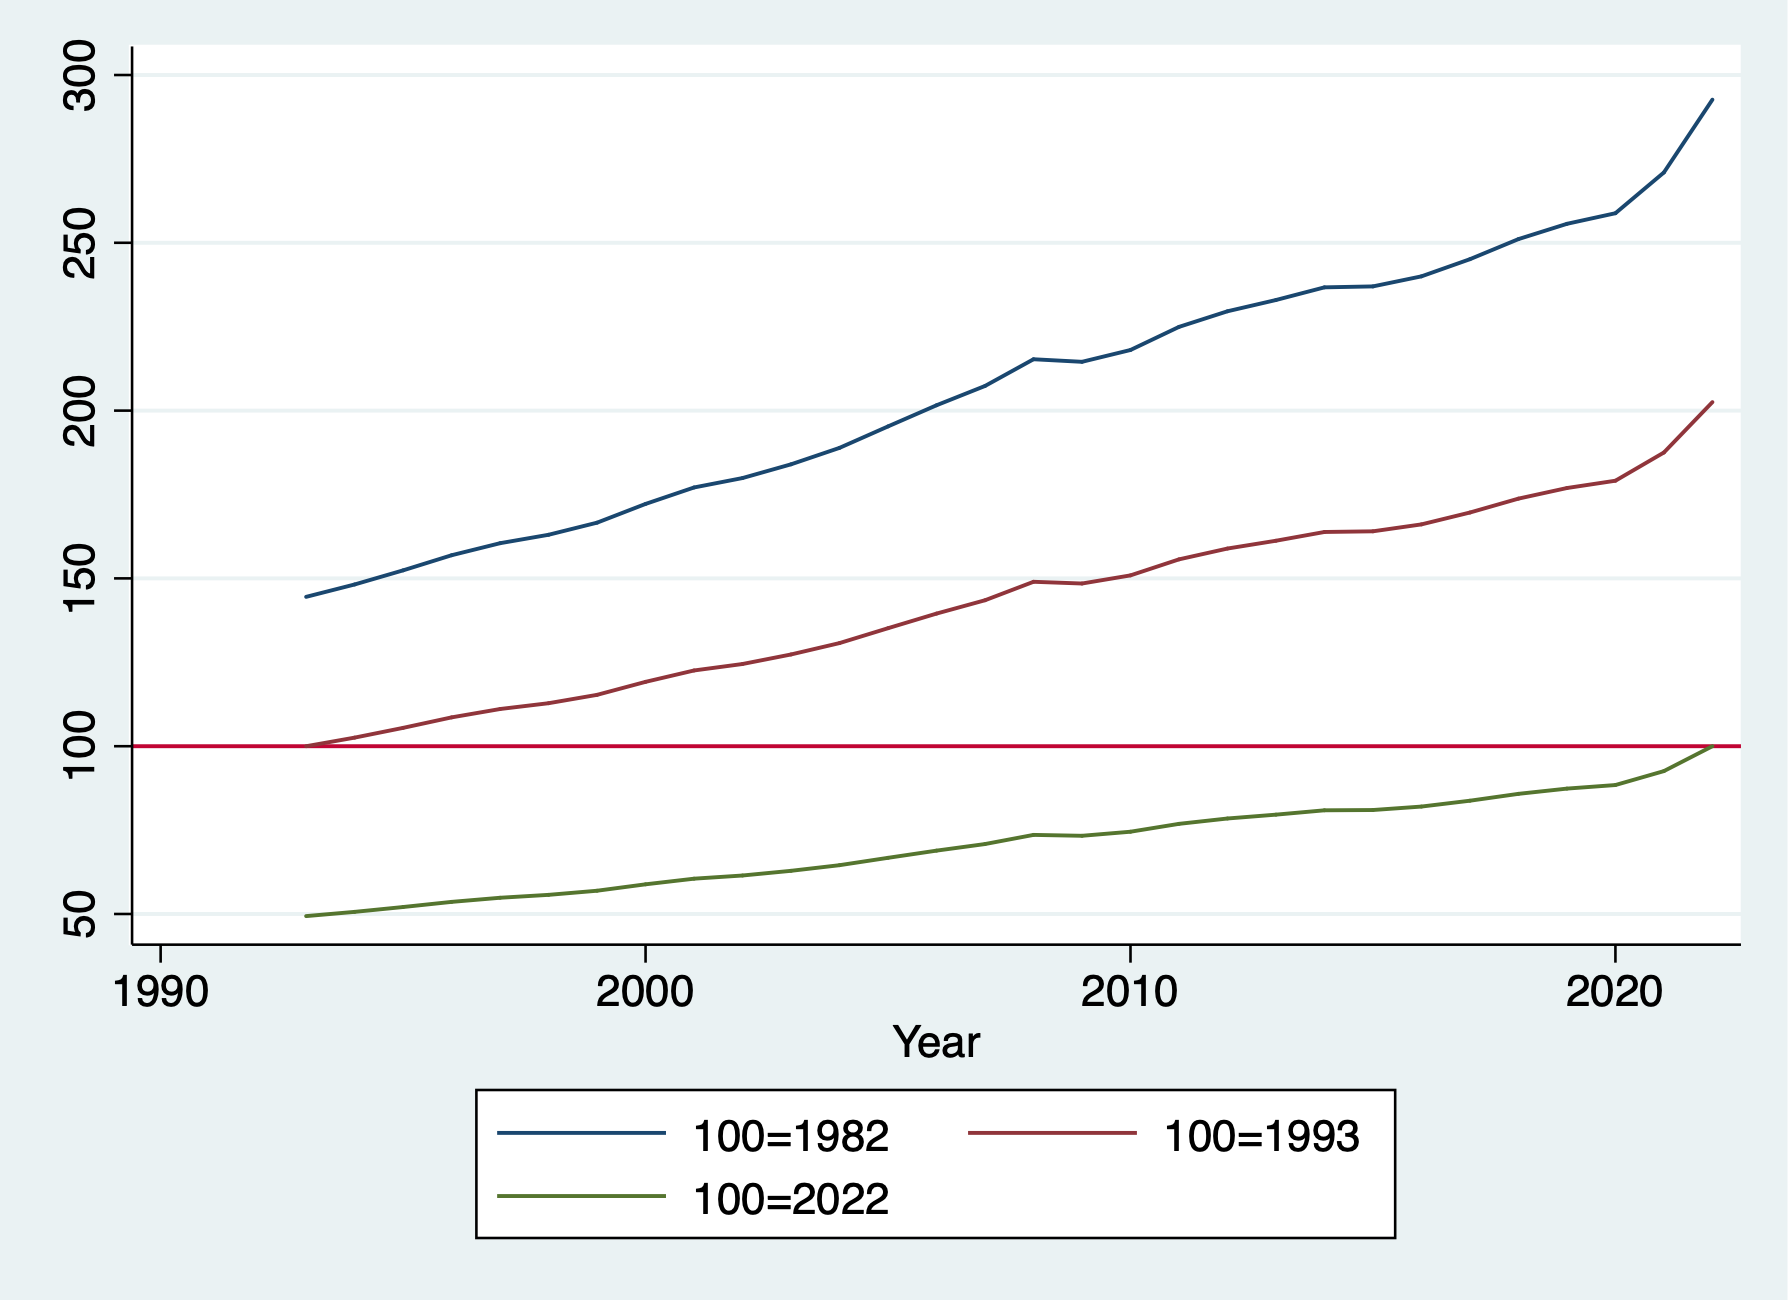
\includegraphics[keepaspectratio]{week8_bls.png}}
\caption{Indexed CPI}
\end{figure}

\section{Computing values within subgroups: Running sums}\label{computing-values-within-subgroups-running-sums}

As we mentioned earlier, when we use \emph{egen sum} vs \emph{gen sum}, we get different
results. \emph{Egen sum()} is similar to \emph{egen total()}, but it can be confusing.
When we use \emph{gen} with \emph{sum()}, we generate a \textbf{RUNNING} sum not a constant of total.

We can generate the tv running sum across all individuals over time

\begin{Shaded}
\begin{Highlighting}[]
\NormalTok{cd }\StringTok{"/Users/Sam/Desktop/Econ 645/Data/Mitchell"}
\KeywordTok{use}\NormalTok{ tv1, }\KeywordTok{clear}
\KeywordTok{generate}\NormalTok{ tvrunsum = }\KeywordTok{sum}\NormalTok{(tv)}
\end{Highlighting}
\end{Shaded}

\begin{verbatim}
/Users/Sam/Desktop/Econ 645/Data/Mitchell
\end{verbatim}

We can generate the tv running sum within an individuals time period

\begin{Shaded}
\begin{Highlighting}[]
\KeywordTok{bysort}\NormalTok{ kidid (dt): }\KeywordTok{generate}\NormalTok{ bytvrunsum=}\KeywordTok{sum}\NormalTok{(tv)}
\end{Highlighting}
\end{Shaded}

We can generate the total sum with an individuals time period

\begin{Shaded}
\begin{Highlighting}[]
\KeywordTok{bysort}\NormalTok{ kidid (dt): }\KeywordTok{egen}\NormalTok{ bytvsum=}\KeywordTok{total}\NormalTok{(tv)}
\end{Highlighting}
\end{Shaded}

We can generate the total sum for all individuals over time

\begin{Shaded}
\begin{Highlighting}[]
\KeywordTok{egen}\NormalTok{ tvsum = }\KeywordTok{total}\NormalTok{(tv)}
\end{Highlighting}
\end{Shaded}

We can also calculate a running average

\begin{Shaded}
\begin{Highlighting}[]
\KeywordTok{bysort}\NormalTok{ kidid (dt): }\KeywordTok{generate}\NormalTok{ bytvrunavg=}\KeywordTok{sum}\NormalTok{(tv)/}\DataTypeTok{\_n}
\end{Highlighting}
\end{Shaded}

We can compute the individual's average average

\begin{Shaded}
\begin{Highlighting}[]
\KeywordTok{bysort}\NormalTok{ kidid (dt): }\KeywordTok{egen}\NormalTok{ bytvavg = }\KeywordTok{mean}\NormalTok{(tv)}
\OtherTok{list}\NormalTok{ kidid tv tv* }\KeywordTok{by}\NormalTok{*, sepby(kidid)}
\end{Highlighting}
\end{Shaded}

\begin{verbatim}
     | kidid   tv   tv   tvrunsum   tvsum   bytvru~m   bytvsum   bytvrun~g   bytvavg |
     |-------------------------------------------------------------------------------|
  1. |     1    1    1          1      38          1         4           1         2 |
  2. |     1    3    3          4      38          4         4           2         2 |
     |-------------------------------------------------------------------------------|
  3. |     2    8    8         12      38          8         8           8         8 |
     |-------------------------------------------------------------------------------|
  4. |     3    2    2         14      38          2        14           2       3.5 |
  5. |     3    5    5         19      38          7        14         3.5       3.5 |
  6. |     3    1    1         20      38          8        14   2.6666667       3.5 |
  7. |     3    6    6         26      38         14        14         3.5       3.5 |
     |-------------------------------------------------------------------------------|
  8. |     4    7    7         33      38          7        12           7         4 |
  9. |     4    1    1         34      38          8        12           4         4 |
 10. |     4    4    4         38      38         12        12           4         4 |
     +-------------------------------------------------------------------------------+
\end{verbatim}

\section{Computing values within subgroups: More examples}\label{computing-values-within-subgroups-more-examples}

There are other useful calculations we can do with subscripting/indexing.
Some do overlap with egen, but it is helpful to know the differences.

\subsection*{Counting}\label{counting}
\addcontentsline{toc}{subsection}{Counting}

Count the number of observations: this can be done with subscripting or egen
depending upon what we want

\begin{Shaded}
\begin{Highlighting}[]
\NormalTok{cd }\StringTok{"/Users/Sam/Desktop/Econ 645/Data/Mitchell"}
\KeywordTok{use}\NormalTok{ tv1, }\KeywordTok{clear}

\NormalTok{*Generate }\KeywordTok{total}\NormalTok{ observation }\FunctionTok{count}\NormalTok{ per individual }\FunctionTok{missing} \KeywordTok{or} \KeywordTok{not} \FunctionTok{missing}\NormalTok{:}
\KeywordTok{bysort}\NormalTok{ kidid (dt): }\KeywordTok{generate}\NormalTok{ idcount=\_N}

\NormalTok{*Generate the }\KeywordTok{total}\NormalTok{ observation without }\FunctionTok{missing}
\KeywordTok{bysort}\NormalTok{ kidid (dt): }\KeywordTok{egen}\NormalTok{ idcount\_nomiss = }\FunctionTok{count}\NormalTok{(tv)}

\NormalTok{*Generate a running }\FunctionTok{count} \KeywordTok{of}\NormalTok{ an observation}
\KeywordTok{bysort}\NormalTok{ kidid (dt): }\KeywordTok{gen}\NormalTok{ idruncount = }\DataTypeTok{\_n}
\OtherTok{list}\NormalTok{, sepby(kidid)}
\end{Highlighting}
\end{Shaded}

\begin{verbatim}
/Users/Sam/Desktop/Econ 645/Data/Mitchell

     +----------------------------------------------------------------------------+
     | kidid          dt   female   wt   tv   vac   idcount   idcoun~s   idrunc~t |
     |----------------------------------------------------------------------------|
  1. |     1   07jan2002        1   53    1     1         2          2          1 |
  2. |     1   08jan2002        1   55    3     1         2          2          2 |
     |----------------------------------------------------------------------------|
  3. |     2   16jan2002        1   58    8     1         1          1          1 |
     |----------------------------------------------------------------------------|
  4. |     3   18jan2002        0   60    2     0         4          4          1 |
  5. |     3   19jan2002        0   63    5     1         4          4          2 |
  6. |     3   21jan2002        0   66    1     1         4          4          3 |
  7. |     3   22jan2002        0   64    6     0         4          4          4 |
     |----------------------------------------------------------------------------|
  8. |     4   10jan2002        1   62    7     0         3          3          1 |
  9. |     4   11jan2002        1   58    1     0         3          3          2 |
 10. |     4   13jan2002        1   55    4     0         3          3          3 |
     +----------------------------------------------------------------------------+
\end{verbatim}

\subsection*{Generate Binaries}\label{generate-binaries}
\addcontentsline{toc}{subsection}{Generate Binaries}

We can generate binary variables to find first and last observations or nth
observation. This differences from id counts, we are generating binaries for
when the qualifier is true.

\begin{Shaded}
\begin{Highlighting}[]
\NormalTok{cd }\StringTok{"/Users/Sam/Desktop/Econ 645/Data/Mitchell"}
\KeywordTok{use}\NormalTok{ tv1, }\KeywordTok{clear}

\NormalTok{*Find individuals with only one observation}
\KeywordTok{bysort}\NormalTok{ kidid (dt): }\KeywordTok{generate}\NormalTok{ singleob = (\_N==1)}

\NormalTok{*Find the first observation }\KeywordTok{of}\NormalTok{ an individual}
\KeywordTok{bysort}\NormalTok{ kidid (dt): }\KeywordTok{generate}\NormalTok{ firstob = (}\DataTypeTok{\_n}\NormalTok{==1)}

\NormalTok{*Find the }\FunctionTok{last}\NormalTok{ observation }\KeywordTok{of}\NormalTok{ an individual }
\KeywordTok{bysort}\NormalTok{ kidid (dt): }\KeywordTok{generate}\NormalTok{ lastob = (}\DataTypeTok{\_n}\NormalTok{==\_N)}
\OtherTok{list}\NormalTok{, sepby(kidid)}
\end{Highlighting}
\end{Shaded}

\begin{verbatim}
/Users/Sam/Desktop/Econ 645/Data/Mitchell

     +--------------------------------------------------------------------------+
     | kidid          dt   female   wt   tv   vac   singleob   firstob   lastob |
     |--------------------------------------------------------------------------|
  1. |     1   07jan2002        1   53    1     1          0         1        0 |
  2. |     1   08jan2002        1   55    3     1          0         0        1 |
     |--------------------------------------------------------------------------|
  3. |     2   16jan2002        1   58    8     1          1         1        1 |
     |--------------------------------------------------------------------------|
  4. |     3   18jan2002        0   60    2     0          0         1        0 |
  5. |     3   19jan2002        0   63    5     1          0         0        0 |
  6. |     3   21jan2002        0   66    1     1          0         0        0 |
  7. |     3   22jan2002        0   64    6     0          0         0        1 |
     |--------------------------------------------------------------------------|
  8. |     4   10jan2002        1   62    7     0          0         1        0 |
  9. |     4   11jan2002        1   58    1     0          0         0        0 |
 10. |     4   13jan2002        1   55    4     0          0         0        1 |
     +--------------------------------------------------------------------------+
\end{verbatim}

We can create binaries depending upon leads and lags too.
Look for a change in vac

\begin{Shaded}
\begin{Highlighting}[]
\NormalTok{cd }\StringTok{"/Users/Sam/Desktop/Econ 645/Data/Mitchell"}
\KeywordTok{use}\NormalTok{ tv1, }\KeywordTok{clear}
\KeywordTok{bysort}\NormalTok{ kidid (dt): }\KeywordTok{generate}\NormalTok{ vacstart=(vac==1) \& (vac[}\DataTypeTok{\_n}\NormalTok{{-}1]==0)}
\KeywordTok{bysort}\NormalTok{ kidid (dt): }\KeywordTok{generate}\NormalTok{ vacend=(vac==1) \& (vac[}\DataTypeTok{\_n}\NormalTok{+1]==0)}
\OtherTok{list}\NormalTok{ kidid dt vac*, sepby(kidid)}
\end{Highlighting}
\end{Shaded}

\begin{verbatim}
/Users/Sam/Desktop/Econ 645/Data/Mitchell

     +---------------------------------------------+
     | kidid          dt   vac   vacstart   vacend |
     |---------------------------------------------|
  1. |     1   07jan2002     1          0        0 |
  2. |     1   08jan2002     1          0        0 |
     |---------------------------------------------|
  3. |     2   16jan2002     1          0        0 |
     |---------------------------------------------|
  4. |     3   18jan2002     0          0        0 |
  5. |     3   19jan2002     1          1        0 |
  6. |     3   21jan2002     1          0        1 |
  7. |     3   22jan2002     0          0        0 |
     |---------------------------------------------|
  8. |     4   10jan2002     0          0        0 |
  9. |     4   11jan2002     0          0        0 |
 10. |     4   13jan2002     0          0        0 |
     +---------------------------------------------+
\end{verbatim}

\subsection*{Fill in Missing}\label{fill-in-missing}
\addcontentsline{toc}{subsection}{Fill in Missing}

Another useful tool that we should use with caution is filling in missings.
This should only really be applied when we have a constant variable that
does not change over time.

\begin{Shaded}
\begin{Highlighting}[]
\NormalTok{cd }\StringTok{"/Users/Sam/Desktop/Econ 645/Data/Mitchell"}
\KeywordTok{use}\NormalTok{ tv2, }\KeywordTok{clear}
\KeywordTok{sort}\NormalTok{ kidid dt}
\OtherTok{list}\NormalTok{, sepby(kidid)}
\end{Highlighting}
\end{Shaded}

\begin{verbatim}
/Users/Sam/Desktop/Econ 645/Data/Mitchell

     +--------------------------------------------+
     | kidid          dt   female   wt   tv   vac |
     |--------------------------------------------|
  1. |     1   07jan2002        1   53    1     1 |
  2. |     1   08jan2002        1   55    3     1 |
     |--------------------------------------------|
  3. |     2   16jan2002        1   58    8     1 |
     |--------------------------------------------|
  4. |     3   18jan2002        0   60    2     0 |
  5. |     3   19jan2002        0    .    .     . |
  6. |     3   21jan2002        0   66    .     1 |
  7. |     3   22jan2002        0   64    6     0 |
     |--------------------------------------------|
  8. |     4   10jan2002        1   62    7     0 |
  9. |     4   11jan2002        1   58    .     . |
 10. |     4   13jan2002        1    .    4     0 |
     +--------------------------------------------+
\end{verbatim}

We can backfill the observation with the last nonmissing observation.
First generate a copy of the variable with missing values.

\begin{Shaded}
\begin{Highlighting}[]
\KeywordTok{generate}\NormalTok{ tvimp1 = tv}
\KeywordTok{bysort}\NormalTok{ kidid (dt): }\KeywordTok{replace}\NormalTok{ tvimp1 = tv[}\DataTypeTok{\_n}\NormalTok{{-}1] }\KeywordTok{if} \FunctionTok{missing}\NormalTok{(tv)}
\OtherTok{list}\NormalTok{ kidid dt tv tvimp1, sepby(kidid)}
\end{Highlighting}
\end{Shaded}

\begin{verbatim}
(3 missing values generated)

(2 real changes made)

     +---------------------------------+
     | kidid          dt   tv   tvimp1 |
     |---------------------------------|
  1. |     1   07jan2002    1        1 |
  2. |     1   08jan2002    3        3 |
     |---------------------------------|
  3. |     2   16jan2002    8        8 |
     |---------------------------------|
  4. |     3   18jan2002    2        2 |
  5. |     3   19jan2002    .        2 |
  6. |     3   21jan2002    .        . |
  7. |     3   22jan2002    6        6 |
     |---------------------------------|
  8. |     4   10jan2002    7        7 |
  9. |     4   11jan2002    .        7 |
 10. |     4   13jan2002    4        4 |
     +---------------------------------+
\end{verbatim}

Notice that we are still missing the 3rd observation for the 3rd kid.
It cannot backfill the 3rd observation from the second observation, since
the second observation is missing. There are a couple of strategies to use
We can generate a new variable like Mitchell.

\begin{Shaded}
\begin{Highlighting}[]
\KeywordTok{generate}\NormalTok{ tvimp2 = tvimp1}
\KeywordTok{bysort}\NormalTok{ kidid (dt): }\KeywordTok{replace}\NormalTok{ tvimp2 = tvimp2[}\DataTypeTok{\_n}\NormalTok{{-}1] }\KeywordTok{if} \FunctionTok{missing}\NormalTok{(tvimp2)}
\OtherTok{list}\NormalTok{ kidid tv tvimp*, sepby(kidid)}
\end{Highlighting}
\end{Shaded}

\begin{verbatim}
(1 missing value generated)

(1 real change made)

     +------------------------------+
     | kidid   tv   tvimp1   tvimp2 |
     |------------------------------|
  1. |     1    1        1        1 |
  2. |     1    3        3        3 |
     |------------------------------|
  3. |     2    8        8        8 |
     |------------------------------|
  4. |     3    2        2        2 |
  5. |     3    .        2        2 |
  6. |     3    .        .        2 |
  7. |     3    6        6        6 |
     |------------------------------|
  8. |     4    7        7        7 |
  9. |     4    .        7        7 |
 10. |     4    4        4        4 |
     +------------------------------+
\end{verbatim}

You can just replace tvimp1 twice instead of generating a new variable, but
that is up to the user. You would use tv{[}\_n-1{]} for the first replace and
tvimp1{[}\_n-1{]} for the second replace.

\subsection*{Interpolation}\label{interpolation}
\addcontentsline{toc}{subsection}{Interpolation}

We may need to interpolate between 2 known values and assume a linear trend.

\begin{Shaded}
\begin{Highlighting}[]
\KeywordTok{generate}\NormalTok{ tvimp3=tv}
\NormalTok{*Interpolate }\KeywordTok{for}\NormalTok{ 1 }\FunctionTok{missing} \OtherTok{value}\NormalTok{ between }\KeywordTok{two}\NormalTok{ known }\KeywordTok{values}
\KeywordTok{bysort}\NormalTok{ kidid (dt): }\KeywordTok{replace}\NormalTok{ tvimp3 = (tv[}\DataTypeTok{\_n}\NormalTok{{-}1]+tv[}\DataTypeTok{\_n}\NormalTok{+1])/2 }\KeywordTok{if} \FunctionTok{missing}\NormalTok{(tv)}
\OtherTok{list}\NormalTok{ kidid tv tvimp3, sepby(kidid)}
\end{Highlighting}
\end{Shaded}

\begin{verbatim}
(3 missing values generated)

(1 real change made)

     +---------------------+
     | kidid   tv   tvimp3 |
     |---------------------|
  1. |     1    1        1 |
  2. |     1    3        3 |
     |---------------------|
  3. |     2    8        8 |
     |---------------------|
  4. |     3    2        2 |
  5. |     3    .        . |
  6. |     3    .        . |
  7. |     3    6        6 |
     |---------------------|
  8. |     4    7        7 |
  9. |     4    .      5.5 |
 10. |     4    4        4 |
     +---------------------+
\end{verbatim}

This is a bit of hard coding, but you can interpolate with more than 1 missing.

\begin{Shaded}
\begin{Highlighting}[]
\KeywordTok{bysort}\NormalTok{ kidid (dt): }\KeywordTok{replace}\NormalTok{ tvimp3 = ((tvimp3[4]{-}tvimp3[1])/3)+tvimp3[}\DataTypeTok{\_n}\NormalTok{{-}1] }\KeywordTok{if} \FunctionTok{missing}\NormalTok{(tvimp3) \& kidid==3}
\OtherTok{list}\NormalTok{ kidid tv tvimp3, sepby(kidid)}
\end{Highlighting}
\end{Shaded}

\begin{verbatim}
(2 real changes made)

     +------------------------+
     | kidid   tv      tvimp3 |
     |------------------------|
  1. |     1    1           1 |
  2. |     1    3           3 |
     |------------------------|
  3. |     2    8           8 |
     |------------------------|
  4. |     3    2           2 |
  5. |     3    .   3.3333333 |
  6. |     3    .   4.6666667 |
  7. |     3    6           6 |
     |------------------------|
  8. |     4    7           7 |
  9. |     4    .         5.5 |
 10. |     4    4           4 |
     +------------------------+
\end{verbatim}

\subsection*{Indicators}\label{indicators}
\addcontentsline{toc}{subsection}{Indicators}

What is we want to find outliers in time-varying differences? We can generate
indicators variables to find when a variable changes more than a set limit.
For example we want to know if the tv viewing habits drop more than 2 hours

\begin{Shaded}
\begin{Highlighting}[]
\NormalTok{cd }\StringTok{"/Users/Sam/Desktop/Econ 645/Data/Mitchell"}
\KeywordTok{use}\NormalTok{ tv1, }\KeywordTok{clear}
\KeywordTok{bysort}\NormalTok{ kidid (dt): }\KeywordTok{generate}\NormalTok{ tvchange = tv[}\DataTypeTok{\_n}\NormalTok{]{-}tv[}\DataTypeTok{\_n}\NormalTok{{-}1]}
\KeywordTok{bysort}\NormalTok{ kidid (dt): }\KeywordTok{generate}\NormalTok{ tvchangerate = ((tv[}\DataTypeTok{\_n}\NormalTok{]{-}tv[}\DataTypeTok{\_n}\NormalTok{{-}1])/tv[}\DataTypeTok{\_n}\NormalTok{{-}1])}
\OtherTok{list}\NormalTok{, sepby(kidid)}
\end{Highlighting}
\end{Shaded}

\begin{verbatim}
/Users/Sam/Desktop/Econ 645/Data/Mitchell


(4 missing values generated)

(4 missing values generated)

     +--------------------------------------------------------------------+
     | kidid          dt   female   wt   tv   vac   tvchange   tvchange~e |
     |--------------------------------------------------------------------|
  1. |     1   07jan2002        1   53    1     1          .            . |
  2. |     1   08jan2002        1   55    3     1          2            2 |
     |--------------------------------------------------------------------|
  3. |     2   16jan2002        1   58    8     1          .            . |
     |--------------------------------------------------------------------|
  4. |     3   18jan2002        0   60    2     0          .            . |
  5. |     3   19jan2002        0   63    5     1          3          1.5 |
  6. |     3   21jan2002        0   66    1     1         -4          -.8 |
  7. |     3   22jan2002        0   64    6     0          5            5 |
     |--------------------------------------------------------------------|
  8. |     4   10jan2002        1   62    7     0          .            . |
  9. |     4   11jan2002        1   58    1     0         -6   -.85714286 |
 10. |     4   13jan2002        1   55    4     0          3            3 |
     +--------------------------------------------------------------------+
\end{verbatim}

Generate an indicator variable to see if tvchange is less than -2. This is not
very helpful with small datasets, but it is important with larger datasets such as the CPS.

\begin{Shaded}
\begin{Highlighting}[]
\KeywordTok{gen}\NormalTok{ tvchangeid=(tvchange \textless{}= {-}2) }\KeywordTok{if}\NormalTok{ !}\FunctionTok{missing}\NormalTok{(tvchange)}
\OtherTok{list}\NormalTok{, sepby(kidid)}
\end{Highlighting}
\end{Shaded}

\begin{verbatim}
(4 missing values generated)

     +-------------------------------------------------------------------------------+
     | kidid          dt   female   wt   tv   vac   tvchange   tvchange~e   tvchan~d |
     |-------------------------------------------------------------------------------|
  1. |     1   07jan2002        1   53    1     1          .            .          . |
  2. |     1   08jan2002        1   55    3     1          2            2          0 |
     |-------------------------------------------------------------------------------|
  3. |     2   16jan2002        1   58    8     1          .            .          . |
     |-------------------------------------------------------------------------------|
  4. |     3   18jan2002        0   60    2     0          .            .          . |
  5. |     3   19jan2002        0   63    5     1          3          1.5          0 |
  6. |     3   21jan2002        0   66    1     1         -4          -.8          1 |
  7. |     3   22jan2002        0   64    6     0          5            5          0 |
     |-------------------------------------------------------------------------------|
  8. |     4   10jan2002        1   62    7     0          .            .          . |
  9. |     4   11jan2002        1   58    1     0         -6   -.85714286          1 |
 10. |     4   13jan2002        1   55    4     0          3            3          0 |
     +-------------------------------------------------------------------------------+
\end{verbatim}

\section{Comparing the by, tsset, xtset commands}\label{comparing-the-by-tsset-xtset-commands}

Another way to find differences within vectors, we can use the tsset or xtset
command to establish the times series (tsset) or panel data (xtset).
We can use our bysort with subscripting/indexing.

\begin{Shaded}
\begin{Highlighting}[]
\NormalTok{cd }\StringTok{"/Users/Sam/Desktop/Econ 645/Data/Mitchell"}
\KeywordTok{use}\NormalTok{ tv1, }\KeywordTok{clear}
\KeywordTok{bysort}\NormalTok{ kidid (dt): }\KeywordTok{generate}\NormalTok{ ltv = tv[}\DataTypeTok{\_n}\NormalTok{{-}1]}
\OtherTok{list}\NormalTok{, sepby(kidid)}
\end{Highlighting}
\end{Shaded}

\begin{verbatim}
/Users/Sam/Desktop/Econ 645/Data/Mitchell


(4 missing values generated)

     +--------------------------------------------------+
     | kidid          dt   female   wt   tv   vac   ltv |
     |--------------------------------------------------|
  1. |     1   07jan2002        1   53    1     1     . |
  2. |     1   08jan2002        1   55    3     1     1 |
     |--------------------------------------------------|
  3. |     2   16jan2002        1   58    8     1     . |
     |--------------------------------------------------|
  4. |     3   18jan2002        0   60    2     0     . |
  5. |     3   19jan2002        0   63    5     1     2 |
  6. |     3   21jan2002        0   66    1     1     5 |
  7. |     3   22jan2002        0   64    6     0     1 |
     |--------------------------------------------------|
  8. |     4   10jan2002        1   62    7     0     . |
  9. |     4   11jan2002        1   58    1     0     7 |
 10. |     4   13jan2002        1   55    4     0     1 |
     +--------------------------------------------------+
\end{verbatim}

\subsection*{tsset}\label{tsset}
\addcontentsline{toc}{subsection}{tsset}

Instead we can establish a time series with \emph{tsset}

We'll need to specify that our cross-sectional groups is kidid.
We'll need to specify our date variable with dt.
We'll need to use the option, daily, to specify that time period is daily
as opposed to weeks, months, years. Or we can specify delta(1) for one day.

We can use the operator \emph{L.var} to specify that we want to a lag of 1 day

\begin{Shaded}
\begin{Highlighting}[]
\NormalTok{cd }\StringTok{"/Users/Sam/Desktop/Econ 645/Data/Mitchell"}
\KeywordTok{use}\NormalTok{ tv1, }\KeywordTok{clear}
\KeywordTok{sort}\NormalTok{ kidid dt}
\KeywordTok{tsset}\NormalTok{ kidid dt, }\FunctionTok{daily}\NormalTok{ delta(1)}
\KeywordTok{generate}\NormalTok{ lagtv = L.tv}
\end{Highlighting}
\end{Shaded}

\begin{verbatim}
/Users/Sam/Desktop/Econ 645/Data/Mitchell

       panel variable:  kidid (unbalanced)
        time variable:  dt, 07jan2002 to 22jan2002, but with gaps
                delta:  1 day

(6 missing values generated)
\end{verbatim}

We can use the operator F.var to specify that we want a lead of 1 day

\begin{Shaded}
\begin{Highlighting}[]
\KeywordTok{generate}\NormalTok{ leadtv = }\FunctionTok{F}\NormalTok{.tv}
\OtherTok{list}\NormalTok{, sepby(kidid)}
\end{Highlighting}
\end{Shaded}

\begin{verbatim}
(6 missing values generated)

     +-------------------------------------------------------------+
     | kidid          dt   female   wt   tv   vac   lagtv   leadtv |
     |-------------------------------------------------------------|
  1. |     1   07jan2002        1   53    1     1       .        3 |
  2. |     1   08jan2002        1   55    3     1       1        . |
     |-------------------------------------------------------------|
  3. |     2   16jan2002        1   58    8     1       .        . |
     |-------------------------------------------------------------|
  4. |     3   18jan2002        0   60    2     0       .        5 |
  5. |     3   19jan2002        0   63    5     1       2        . |
  6. |     3   21jan2002        0   66    1     1       .        6 |
  7. |     3   22jan2002        0   64    6     0       1        . |
     |-------------------------------------------------------------|
  8. |     4   10jan2002        1   62    7     0       .        1 |
  9. |     4   11jan2002        1   58    1     0       7        . |
 10. |     4   13jan2002        1   55    4     0       .        . |
     +-------------------------------------------------------------+
\end{verbatim}

\subsection*{xtset}\label{xtset}
\addcontentsline{toc}{subsection}{xtset}

We can establish a panel series with \emph{xtset}

We'll need to specify that our cross-sectional group is kidid.
We'll need to specify our time period is dt.
We'll use a delta of 1 to specify that the differnce is 1 day.
Or, we can use \emph{daily}, as well

Generate a lag with the l.var operator and generate a lead with the f.var

\begin{Shaded}
\begin{Highlighting}[]
\NormalTok{cd }\StringTok{"/Users/Sam/Desktop/Econ 645/Data/Mitchell"}
\KeywordTok{use}\NormalTok{ tv1, }\KeywordTok{clear}
\KeywordTok{sort}\NormalTok{ kidid dt}
\NormalTok{xtset kidid dt, }\FunctionTok{daily}\NormalTok{ delta(1)}
\KeywordTok{generate}\NormalTok{ lagtv = }\OtherTok{l}\NormalTok{.tv}
\KeywordTok{generate}\NormalTok{ leadtv = f.tv}
\end{Highlighting}
\end{Shaded}

\begin{verbatim}
/Users/Sam/Desktop/Econ 645/Data/Mitchell

       panel variable:  kidid (unbalanced)
        time variable:  dt, 07jan2002 to 22jan2002, but with gaps
                delta:  1 day

(6 missing values generated)

(6 missing values generated)
\end{verbatim}

What do you notice? You can see that there are some leads and lags missing.
Why? Because there is an unbalance panel and the daily differences cannot be
computed if we are missing days. In this case, we can use the bysort with
subscripting indexing

\begin{Shaded}
\begin{Highlighting}[]
\OtherTok{list}\NormalTok{, sepby(kidid)}
\KeywordTok{bysort}\NormalTok{ kidid (dt): }\KeywordTok{gen}\NormalTok{ bylagtv=tv[}\DataTypeTok{\_n}\NormalTok{{-}1]}
\KeywordTok{bysort}\NormalTok{ kidid (dt): }\KeywordTok{gen}\NormalTok{ byleadtv=tv[}\DataTypeTok{\_n}\NormalTok{+1]}
\OtherTok{list}\NormalTok{, sepby(kidid)}
\end{Highlighting}
\end{Shaded}

\begin{verbatim}
     | kidid          dt   female   wt   tv   vac   lagtv   leadtv |
     |-------------------------------------------------------------|
  1. |     1   07jan2002        1   53    1     1       .        3 |
  2. |     1   08jan2002        1   55    3     1       1        . |
     |-------------------------------------------------------------|
  3. |     2   16jan2002        1   58    8     1       .        . |
     |-------------------------------------------------------------|
  4. |     3   18jan2002        0   60    2     0       .        5 |
  5. |     3   19jan2002        0   63    5     1       2        . |
  6. |     3   21jan2002        0   66    1     1       .        6 |
  7. |     3   22jan2002        0   64    6     0       1        . |
     |-------------------------------------------------------------|
  8. |     4   10jan2002        1   62    7     0       .        1 |
  9. |     4   11jan2002        1   58    1     0       7        . |
 10. |     4   13jan2002        1   55    4     0       .        . |
     +-------------------------------------------------------------+

(4 missing values generated)

(4 missing values generated)

     +----------------------------------------------------------------------------------+
     | kidid          dt   female   wt   tv   vac   lagtv   leadtv   bylagtv   byleadtv |
     |----------------------------------------------------------------------------------|
  1. |     1   07jan2002        1   53    1     1       .        3         .          3 |
  2. |     1   08jan2002        1   55    3     1       1        .         1          . |
     |----------------------------------------------------------------------------------|
  3. |     2   16jan2002        1   58    8     1       .        .         .          . |
     |----------------------------------------------------------------------------------|
  4. |     3   18jan2002        0   60    2     0       .        5         .          5 |
  5. |     3   19jan2002        0   63    5     1       2        .         2          1 |
  6. |     3   21jan2002        0   66    1     1       .        6         5          6 |
  7. |     3   22jan2002        0   64    6     0       1        .         1          . |
     |----------------------------------------------------------------------------------|
  8. |     4   10jan2002        1   62    7     0       .        1         .          1 |
  9. |     4   11jan2002        1   58    1     0       7        .         7          4 |
 10. |     4   13jan2002        1   55    4     0       .        .         1          . |
     +----------------------------------------------------------------------------------+
\end{verbatim}

\subsection*{What is the difference? xtset vs tsset}\label{what-is-the-difference-xtset-vs-tsset}
\addcontentsline{toc}{subsection}{What is the difference? xtset vs tsset}

From Nick Cox:
xtset allows a panel identifier only. tsset allows a time identifier only.
Where they overlap is when two variables are supplied in which case the first
is treated as a panel identifier and the second as a time variable.

\section{Exercises}\label{exercises}

Let's grab the CPS and generate subgroup analysis. We will be using unweighted data for simplicity
1. What are the average wages by sex?
2. What are average wages by state
3. What are the median wages by sex
4. What are the median wages by state
5. What is the 75th percentile of wages by race?
6. What is the 25th percentile of wages by marital status?

\begin{Shaded}
\begin{Highlighting}[]
\KeywordTok{use} \StringTok{"/Users/Sam/Desktop/Econ 645/Data/CPS/jun23pub.dta"}\NormalTok{,}\KeywordTok{replace}
\end{Highlighting}
\end{Shaded}

Use bysort state: egen totalvar=total(var1)

Mitchell, N.M. (2020). \emph{Data Management Using Stata: A Practical Handbook}. (2nd ed.). Stata Press.

UCLA Advanced Research Computing. (2025). \emph{How can I access information stored after I run a command in Stata.} Retrieved from \url{https://stats.oarc.ucla.edu/stata/faq/how-can-i-access-information-stored-after-i-run-a-command-in-stata-returned-results/}

Wooldridge (2009). \emph{Introductory Econometrics: A Modern Approach}. (4th ed.). South-Western Cengage Learning.

\bibliography{book.bib,packages.bib}

\end{document}
